\section{Systém iterovaných funkcí}\label{sec:ifs}

V předchozí části kapitoly jsme viděli, jak lze fraktální objekty efektivně popisovat pomocí L-systémů, kde struktura vzniká paralelním přepisováním symbolů a~jejich vizualizace se provádí prostřednictvím želví grafiky. Tento přístup nám umožňoval popsat určitou skupinu fraktálů, nicméně pro jiné fraktály by se nám hodil vhodnější popis jejich konstrukce. Např. Sierpińského trojúhelník lze generovat pomocí L-systému, nicméně v~sekci~\ref{sec:sobepodobnost} o~soběpodobnosti jsme si jej záváděli spíše pomocí opakované aplikace určitých geometrických transformací (ač jsme neuvedli jejich explicitní vyjádření). Ty si později zavedeme jako tzv. \emph{systémy iterovaných funkcí}\index{systém iterovaných funkcí}.

Nejdříve se podíváme trochu více na matematickou podstatu. Hodně záležitostí jsme si již rozebrali v~kapitole~\ref{chapter:hausdorffuv-mp} o~Hausdorffově metrickém prostoru\index{Hausdorffův metrický prostor}\index{metrický prostor!Hausdorffův}, který zde bude hrát významnou roli. Pro související matematickou teorii, kterou zde dále budeme vykládat, doporučuji knihu \cite{Barnsley1993}.

\subsection{Kontrakce na Hausdorffově metrickém prostoru}\label{subsec:hausdorffuv-mp-kontrakce}

V minulých kapitolách jsme se často zaměřovali na lipschitzovská a~bilipschitzovská zobrazení. V~tomto případě nás budou speciálně zajímat tzv. \emph{kontrakce}\index{kontrakce}\index{zobrazení!kontraktivní}. Těmto termínům a~faktům s~nimi souvisejícími jsme se krátce věnovali v~podsekci~\ref{subsec:lipschitzovska-zobrazeni}.

Připomeňme, že lipschitzovskost rovnou implikuje spojitost zobrazení v~libovolném metrickém prostoru $(X,\varrho)$. Ještě než však začneme, podíváme se na alternativní definici Hausdorffovy metriky, která se nám dále bude hodit.
\begin{theorem}[Alternativní definice Hausdorffovy metriky]\label{thm:alternativni-hausdorffova-metrika}
    Nechť $(X,\varrho)$ je metrický prostor. Pro každé $A,B\in\hyperspace(X)$ platí
    \[\hausdorffmetric(A,B)=\max\set{\sup_{x\in A}\varrho(x,B),\sup_{y\in B}\varrho(y,A)}.\]
\end{theorem}
\begin{proof}
    Nechť je dáno $\varepsilon>0$ takové, že $\varepsilon\geqslant\hausdorffmetric(A,B)$. Pak $A\subseteq(B)_\varepsilon$ a~$B\subseteq(A)_\varepsilon$, tzn.
    \[\varepsilon\geqslant\max\set{\sup_{x\in A}\varrho(x,B),\sup_{y\in B}\varrho(y,A)}.\]
    Naopak zvolíme-li $0<\varepsilon\leqslant\hausdorffmetric(A,B)$, pak určitě platí alespoň jedna z~nerovností:
    \[\varepsilon\leqslant\sup_{x\in A}\varrho(x,B)\quad\text{nebo}\quad\varepsilon\leqslant\sup_{y\in B}\varrho(y,A).\]
    Tedy
    \[\varepsilon\leqslant\max\set{\sup_{x\in A}\varrho(x,B),\sup_{y\in B}\varrho(y,A)}.\]
    Z~toho dostáváme závěr tvrzení.
\end{proof}

Jako první se podíváme na trojici pomocných lemmat.
\begin{lemma}\label{lem:spojitost-a-hyperprostor}
    Nechť $\mapping{f}{X}{X}$ je spojisté zobrazení v~metrickém prostoru $(X,\varrho)$. Pak pro každé $S\in\hyperspace(X)$ platí $f(S)\in\hyperspace(X)$.
\end{lemma}
\begin{proof}
    Nechť $S\in\hyperspace(X)$. Zjevně platí $f(S)\neq\emptyset$. Pro důkaz kompaktnosti $f(S)$ uvažujme posloupnost $\set{x_n}_{n=1}^\infty$, kde $x_i\in S$ pro každé $i\in\N$. Protože $S$ je kompaktní, existuje posloupnost indexů $\set{n_k}_{k=1}^\infty$, taková, že $x_{n_k}\to x\in S$. Ze spojitosti zobrazení $f$ však plyne, že pak $\set{f(x_{n_k})}_{k=1}^\infty$ je podposloupností posloupnosti $\set{f(x_n)}_{n=1}^\infty$ a~$f(x_{n_k})\to f(x)$, tedy i~$f(S)$ je kompaktní.
\end{proof}
\begin{lemma}\label{lem:kontrakce-a-hyperprostor}
    Nechť $\mapping{f}{X}{X}$ je kontrakce na metrickém prostoru $(X,\varrho)$ s~faktorem $0<K<1$. Pak $\mapping{f}{\hyperspace(X)}{\hyperspace(X)}$ je kontrakce na Hausdorffově metrickém prostoru s~faktorem $K$.
\end{lemma}
(Převzato z~\citep[str. 79]{Barnsley1993}.)
\begin{proof}
    Z~předchozího lemmatu~\ref{lem:spojitost-a-hyperprostor} víme, že $f(S)\in\hyperspace(X)$ pro každé $S\in\hyperspace(X)$. Mějme množiny $A,B\in\hyperspace(X)$. Pak
    \begin{align*}
        \varrho(f(A),f(B))&=\inf\set{\varrho(f(x),f(y))\mid x\in A\;,\;y\in B}\\
        &\leqslant\inf\set{K\cdot\varrho(x,y)\mid x\in A\;,\;y\in B}\\
        &=K\cdot\inf\set{\varrho(x,y)\mid x\in A\;,\;y\in B}\\
        &=K\cdot\varrho(A,B).
    \end{align*}
    Tedy celkově
    \begin{align*}
        \hausdorffmetric(f(A),f(B))&=\inf\set{\delta>0\mid f(A)\subseteq(f(B))_\delta\land f(B)\subseteq(f(A))_\delta}\\
        &=\max\set{\sup_{x\in A}\varrho(f(x),f(B)),\sup_{y\in B}\varrho(f(y),f(A))}\\
        &=\max\set{\sup_{x\in A}\inf_{y\in B}\varrho(f(x),f(y)),\sup_{y\in B}\inf_{x\in A}\varrho(f(y),f(x))}\\
        &\leqslant K\max\set{\sup_{x\in A}\inf_{y\in B}\varrho(f(x),f(y)),\sup_{y\in B}\inf_{x\in A}\varrho(f(y),f(x))}\\
        &=K\hausdorffmetric(A,B).
    \end{align*}
    Druhá rovnost plyne z~věty~\ref{thm:alternativni-hausdorffova-metrika}.
\end{proof}
(Převzato a~upraveno z~\citep[str. 79]{Barnsley1993}.)
\begin{lemma}\label{lem:hausdorffova-metrika-odhad-sjednoceni}
    Pro každé množiny $A,B,C,D\in\hyperspace(X)$, kde $(X,\varrho)$ je metrický prostor, platí
    \[\hausdorffmetric(A\cup B,C\cup D)\leqslant\max\set{\hausdorffmetric(A,C),\hausdorffmetric(B,D)}.\]
\end{lemma}
\begin{proof}
    Budeme vycházet z~alternativní definice Hausdorffovy metriky, jejíž ekvivalenci s~původní definicí jsme dokázali výše (viz věta~\ref{thm:alternativni-hausdorffova-metrika}). Pro $\varrho(x,A\cup B)$ platí následující odhad:
    \[\varrho(x,A\cup B)=\min\set{\inf_{y\in A}\varrho(x,y),\inf_{z\in B}\varrho(x,z)}\leqslant\inf_{y\in A}\varrho(x,y)=\varrho(x,A).\]
    Z~toho pak máme
    \[\sup_{x\in A}\varrho(x,C\cup D)\leqslant\sup_{x\in A}\inf_{y\in C}\varrho(x,y)=\varrho(x,A)\leqslant\hausdorffmetric(A,C)\]
    a~tedy
    \[\sup_{x\in A\cup B}\varrho(x,C\cup D)\leqslant\max\set{\hausdorffmetric(A,C),\hausdorffmetric(B,D)}.\]
    Stejný odhad lze získat i~pro $\sup_{x\in C\cup D}\varrho(x,A\cup B)$:
    \begin{align*}
        \sup_{x\in C\cup D}\varrho(x,A\cup B)&=\max\set{\sup_{x\in C}\varrho(x,A\cup B),\sup_{x\in D}\varrho(x,A\cup B)}\\
        &\leqslant\max\set{\hausdorffmetric(C,A),\hausdorffmetric(D,B)}=\max\set{\hausdorffmetric(A,C),\hausdorffmetric(B,D)}.
    \end{align*}
    Tedy celkově lze psát
    \begin{align*}
        \hausdorffmetric(A\cup B,C\cup D)&=\max\set{\sup_{x\in A\cup B}\varrho(x,C\cup D),\sup_{x\in C\cup D}\varrho(x,A\cup B)}\\
        &\leqslant\max\set{\hausdorffmetric(A,C),\hausdorffmetric(B,D)}.
    \end{align*}
\end{proof}

Dvojice lemmat~\ref{lem:spojitost-a-hyperprostor} a~\ref{lem:kontrakce-a-hyperprostor} nám v~podstatě říká, že obrazem kompaktní množiny v~kontraktivním zobrazení\index{zobrazení!kontraktivní}\index{kontraktivní zobrazení} je opět kompaktní množina a~že "kontraktivita" zobrazení definovaného na libovolném metrickém prostoru $(X,\varrho)$ se zachovává na hyperprostoru. Tento výsledek se nám bude později hodit, neboť neboť jak již bylo zmíněno na začátku, některé fraktály lze konstruovat pomocí opakované aplikace určitých geometrických tranformací. Jak lze nejspíše z~dosavadního výkladu tušit, budeme pracovat právě s~kontrakcemi.
\begin{definition}[Systém iterovaných funkcí]\label{def:system-iterovanych-funkci}
    \emph{Systém iterovaných funkcí}\index{systém iterovaných funkcí}, zkráceně IFS (z anglického \emph{iterated function system}\index{iterated function system}), na metrickém prostoru $(X,\varrho)$ je konečná množina kontrakcí
    \[\set{\mapping{\psi_i}{X}{X}\mid 1\leqslant i\leqslant n}\]
    s~faktory $K_i$. Kontraktivním faktorem IFS je číslo $K=\max\set{K_i\mid 1\leqslant i\leqslant n}$.
\end{definition}
Zatím není zcela zjevné, proč definujeme pro IFS kontraktivní faktor jako maximum z~faktorů všech kontrakcí v~něm obsažených (byť to může působit do jisté míry intuitivně). Odpověď na tuto otázku nám poskytne následující věta~\ref{thm:sjednoceni-kontrakci}.
\begin{theorem}\label{thm:sjednoceni-kontrakci}
    Nechť $\set{\psi_1,\psi_2,\ldots,\psi_n}$ je IFS na metrickém prostoru $(X,\varrho)$ s~kontraktivním faktorem\index{faktor}\index{kontraktivní faktor}\index{faktor!kontraktivní} $0<K<1$. Pak zobrazení $\mapping{\Psi}{\hyperspace(X)}{\hyperspace(X)}$ definované předpisem
    \[\Psi(A)=\bigcup_{i=1}^n\psi_i(A)\]
    pro $A\in\hyperspace(X)$ je kontrakce na $(\hyperspace(X),\hausdorffmetric)$ s~faktorem $K$.
\end{theorem}
(Převzato z~\citep[str. 81]{Barnsley1993}.)
\begin{proof}
    Důkaz tvrzení lze provést indukcí podle $n$. V~případě, kdy $n=1$ je situace triviální. Pro $n=2$ zvolme množiny $A,B\in\hyperspace(X)$. Pak
    \begin{align*}
        \hausdorffmetric(\psi_1(A)\cup\psi_2(A),\psi_1(B)\cup\psi_2(B))&\leqslant\max\set{\hausdorffmetric(\psi_1(A),\psi_1(B)),\hausdorffmetric(\psi_2(A),\psi_2(B))}\\
        &\leqslant\max\set{K_1\hausdorffmetric(A,B),K_2\hausdorffmetric(A,B)}\\
        &\leqslant K\hausdorffmetric(A,B),
    \end{align*}
    kde druhá nerovnost plyne z~lemmatu~\ref{lem:hausdorffova-metrika-odhad-sjednoceni}. Nyní ukážeme, že zobrazení $\Psi
    $ definované předpisem $\Psi(A)=\bigcup_{i=1}^n\psi_i(A)$ je kontrakce. Mějme opět množiny $A,B\in\hyperspace(X)$. Pak
    \begin{align*}
        \hausdorffmetric(\Psi(A),\Psi(B))&=\hausdorffmetric\left(\left(\bigcup_{i=1}^{n-1}\psi_i(A)\right)\cup\psi_n(A),\left(\bigcup_{i=1}^{n-1}\psi_i(B)\right)\cup\psi_n(B)\right)\\
        &\leqslant\max\set{\hausdorffmetric\left(\bigcup_{i=1}^{n-1}\psi_i(A),\bigcup_{i=1}^{n-1}\psi_i(B)\right),\hausdorffmetric(\psi_n(A)\cup\psi_n(B))}\\
        &\stackrel{\text{I.P.}}{\leqslant}\max\set{K\hausdorffmetric(A,B),K_n\hausdorffmetric(A,B)}\leqslant K\hausdorffmetric(A,B).
    \end{align*}
\end{proof}
\begin{remark}
    Dodejme, že dále v~textu budeme používat značení $\Psi^{\circ n}$ definované induktivně:
    \begin{align*}
        \Psi^{\circ 0}&=\id,\\
        \Psi^{\circ n}&=\Psi\circ\Psi^{\circ(n-1)}\;,\;n\in\N.
    \end{align*}
    Tzn.~pro libovolnou množinu $B\in\hyperspace(X)$ je
    \[\Psi^{\circ 0}(B)=B\quad\text{a}\quad\Psi^{\circ n}(B)=\Psi(\Psi^{\circ(n-1)}(B)).\]
\end{remark}

S kontrakcemi se pojí známá věta z~matematické analýzy, která se nazývá \emph{Banachova věta o~pevném bodě} (viz~\ref{thm:banach}).
\begin{definition}[Pevný bod]\label{def:pevny-bod}
    Bod $x\in X$ se nazývá pevným bodem zobrazení $\mapping{f}{X}{X}$, pokud $f(x)=x$.
\end{definition}
\begin{theorem}[Banachova věta o~pevném bodě]\label{thm:banach}
    Nechť $(X,\varrho)$ je úplný metrický prostor a~zobrazení $\mapping{f}{X}{X}$ je kontrakce. Pak existuje právě jeden pevný bod $x\in X$ zobrazení $f$. Navíc volíme-li $x_0\in\N$ libovolně a~$x_n=f(x_{n-1})$ pro každé $n\in\N$, pak $x_n\to x$.
\end{theorem}
\begin{proof}
    Podle předpokladu je $f$ kontrakce s~faktorem $K$. Zvolme $x_0\in X$ a~dále pro každé $n\in\N$ položme $x_n=f(x_{n-1})$. Ukážeme, že takto definovaná posloupnost budů má limitu. Podle předpokladu je $(X,\varrho)$ úplný metrický prostor, tedy stačí ukázat, že posloupnost $\set{x_n}_{n=1}^\infty$ je cauchyovská. Pro vzdálenosti dvou po sobě jdoucích členů platí
    \begin{align*}
        \varrho(x_1,x_2)&=\varrho(f(x_0),f(x_1))\leqslant K\varrho(x_0,x_1),\\
        \varrho(x_2,x_3)&=\varrho(f(x_1),f(x_2))\leqslant K\varrho(x_1,x_2)\leqslant K^2\varrho(x_0,x_1),\\
        \varrho(x_3,x_4)&=\varrho(f(x_2),f(x_3))\leqslant K\varrho(x_2,x_3)\leqslant K^3\varrho(x_0,x_1),\\
        &\vdots\\
        \varrho(x_i,x_{i+1})&=\varrho(f(x_{i-1}),f(x_i))\leqslant K\varrho(x_{i-1},x_i)\leqslant K^i\varrho(x_0,x_1).\\
        &\vdots
    \end{align*}
    Pro odhadnutí vzdálenosti dvojice členů, které nejdou nutně bezprostředně po sobě použijeme trojúhelníkovou nerovnost. Volme $n,m\in\N$, pričemž $m>n$. Pak lze psát
    \begin{align*}
        \varrho(x_n,x_m)&\leqslant\sum_{i=n}^{m-1}\varrho(x_i,x_{i+1})\leqslant\sum_{i=n}^{m-1}K^i\varrho(x_0,x_1)=K^n\varrho(x_0,x_1)\sum_{i=1}^{m-n-1}K^i\\
        &=K^n\varrho(x_0,x_1)\cdot\dfrac{1-K^{n-m}}{K-1}.
    \end{align*}
    Výraz na pravé straně má pro $n\to\infty$ limitu $0$, tedy posloupnost $\set{x_n}_{n=1}^\infty$ je cauchyovská a~má limitu $x\in X$. Dále ze spojitosti funkce $f$ (neboť je lipschitzovská) plyne
    \[x=\lim_{n\to\infty}x_{n+1}=\lim_{n\to\infty}f(x_n)=f(x),\]
    tedy $x\in X$ je pevným bodem $f$. Jednoznačnost pevného bodu $x$ lze ukázat sporem. Pokud by existoval další pevný bod $y\neq x$, pak
    \[\varrho(x,y)=\varrho(f(x),f(y))\leqslant K\varrho(x,y).\]
    Protože $\varrho(x,y)>0$, musí být $K\geqslant 1$, což je spor s~předpokladem, že $f$ je kontrakce.
\end{proof}
Speciálně pro zobrazení $\Psi$ definované ve větě~\ref{thm:sjednoceni-kontrakci} nám Banachova věta~\ref{thm:banach} nejen říká, že má právě jeden pevný bod $A\in\hyperspace(X)$, tzn. $\Psi(A)=A$, ale zároveň udává způsob, jak daný pevný bod nalézt. Stačí opakovaně iterovat dané zobrazení.
\begin{definition}[Atraktor]\label{def:atraktor}
    Pevný bod $A\in\hyperspace(X)$ zobrazení $\Psi$ definovaného ve větě~\ref{thm:sjednoceni-kontrakci} pro libovolné IFS se nazývá \emph{atraktor}\index{atraktor}.
\end{definition}
Z Banachovy věty speciálně plyne, že atraktor $A$ libovolného IFS lze určit jako následující limitu:
\[A=\lim_{n\to\infty}\Psi^{\circ n}(B),\]
kde $B\in\hyperspace(X)$. Zajímavostí je fakt, že výsledný atraktor $A$ je zcela nezávislý na volbě množiny $B$. Tento fakt si ještě přiblížíme v~podsekci~\ref{subsec:fraktaly-ifs}.

V dalším textu budeme pracovat především s~afinními zobrazeními v~$\R^n$ se standardní eukleidovskou metrikou. Připomeňme si zde, že afinním zobrazením rozumíme jakékoliv zobrazení $\mapping{f}{X}{X}$, takové, že
\[f(x)=\mat{A}x+b,\]
kde $b\in X$ a~$\mat{A}$ je regulární matice. O~afinnitách lze též dokázat řadu zajímavých tvrzení, avšak tyto záležitosti již spadají spíše do oblasti lineární algebry. Nicméně v~případě každé z~afinnit, které zde dále uvidíme, se čtenář může celkem snadno přesvědčit, že se skutečně jedná o~kontrakci.

\subsection{Fraktály generované pomocí IFS}\label{subsec:fraktaly-ifs}

V předešlé podsekci~\ref{subsec:hausdorffuv-mp-kontrakce} jsme se společně podívali na některé důležité poznatky týkající se kontrakcí a~Hausdorffova metrického prostoru (viz kapitola~\ref{chapter:hausdorffuv-mp}). Na některá dokázaná tvrzení se zde budeme odkazovat.

Protože pracujeme s~fraktálními útvary v~rovině, tj. $\R^2$, afinní zobrazení, s nimiž budeme pracovat, budou mít tvar
\begin{equation}\label{eq:afinita-v-R2}
    \psi\left(\begin{matrix}
        x\\
        y
    \end{matrix}\right)=\underbrace{\left(\begin{matrix}
        a~& b\\
        c & d
    \end{matrix}\right)}_{\mat{A}}\left(\begin{matrix}
        x\\
        y
    \end{matrix}\right)+\left(\begin{matrix}
        e\\
        f
    \end{matrix}\right).
\end{equation}
Připomeňme, že matice $\mat{A}$ je regulární. Podíváme se na některé fraktály, které jsme již viděli v~úvodní kapitole~\ref{chapter:uvod_do_fraktalu} v~sekci~\ref{sec:sobepodobnost}. Jiný způsob generování těchto a~mnohých jiných fraktálních útvarů nám poskytují L-systémy, které jsme si ilustrovali v~sekci~\ref{sec:L-systemy}.

Znovu se podívejme na asi jeden z~nejznáměnších fraktálů z~této kategorie -- Sierpińského trojúhelník. Jeho konstrukce lze docílit pomocí IFS $\set{\omega_1,\omega_2,\omega_3}$, přičemž $\mapping{\omega_1,\omega_2,\omega_3}{\R^2}{\R^2}$ a~jednotlivé kontrakce jsou definovány následujícími předpisy:
\begin{align*}
    \omega_1\left(\begin{matrix}
        x\\
        y
    \end{matrix}\right)&=\left(\begin{matrix}
        1/2 & 0\\
        0 & 1/2
    \end{matrix}\right)\left(\begin{matrix}
        x\\
        y
    \end{matrix}\right)+\left(\begin{matrix}
        0\\
        0
    \end{matrix}\right),\\
    \omega_2\left(\begin{matrix}
        x\\
        y
    \end{matrix}\right)&=\left(\begin{matrix}
        1/2 & 0\\
        0 & 1/2
    \end{matrix}\right)\left(\begin{matrix}
        x\\
        y
    \end{matrix}\right)+\left(\begin{matrix}
        1/2\\
        0
    \end{matrix}\right),\\
    \omega_3\left(\begin{matrix}
        x\\
        y
    \end{matrix}\right)&=\left(\begin{matrix}
        1/2 & 0\\
        0 & 1/2
    \end{matrix}\right)\left(\begin{matrix}
        x\\
        y
    \end{matrix}\right)+\left(\begin{matrix}
        1/4\\
        \sqrt{3}/4
    \end{matrix}\right).
\end{align*}
Tedy zobrazení $\mapping{\Omega}{\hyperspace(\R^2)}{\hyperspace(\R^2)}$ definujeme jako
\[\Omega(A)=\omega_1(A)\cup\omega_2(A)\cup\omega_3(A),\]
kde $A\in\hyperspace(\R^2)$. Připomeňme, že takto definované $\Omega$ je (podle věty~\ref{thm:sjednoceni-kontrakci}) kontrakce a~tedy z~Banachovy věty o~pevném bodě plyne (viz věta~\ref{thm:banach}), že má právě jeden atraktor, tj. množinu $A\in\hyperspace(\R^2)$ takovou, že platí $A=\Omega(A)$. Kontraktivní faktor tohoto (ani jiného) IFS nás vyloženě zajímat nemusí, avšak není těžké jej dopočítat. Např. zde je celkem zjevné, že $K=1/2$. Užitečnější je však pro nás fakt, že atraktor $A$ lze určit jako
\[A=\lim_{n\to\infty}\Omega^{\circ n}(B),\]
kde $B\in\hyperspace(\R^2)$. V~našem případě je počátečním útvarem rovnostranný trojúhelník $T$, jehož vrcholy mají souřadnice
\[\left(\begin{matrix}
    0\\
    0
\end{matrix}\right),\;\left(\begin{matrix}
    1\\
    0
\end{matrix}\right),\;\left(\begin{matrix}
    1/2\\
    \sqrt{3}/2
\end{matrix}\right).\]
Prvních několik iterací zobrazení $\Omega$ si lze prohlédnout na obrázku~\ref{fig:iterace-zobrazeni-omega-sierpinskeho-trojuhelnik}. Sierpińského trojúhelník je tedy atraktorem zobrazení $\Omega$.

Zajímavostí je, že atraktor daného IFS je zcela nezávislý na volbě počátečního útvaru. Ač je tedy běžné, že v~případě Sierpińského trojúhelníka začínáme s~rovnostranným trojúhelníkem, faktem je, že je zcela lhostejné\footnote{Z formálního hlediska je třeba, aby se jednalo o~kompaktní neprázdnou množinu, nicméně v~$\R^n$ stačí pro tento účel uvažovat všechny neprázdné množiny, které jsou \emph{uzavřené a~omezené} (viz věta~\ref{thm:heine-borel})}, s jakým útvarem začneme (viz obrázek~\ref{fig:iterace-zobrazeni-omega-sierpinskeho-trojuhelnik-jiny-poc-utvar}).

Vypisovat explicitně dané kontrakce je sice formálně žádoucí, nicméně dosti nepraktické. Dále tedy budeme hodnoty jednotlivých koeficientů $a,b,\ldots,f$ (viz \eqref{eq:afinita-v-R2}) zapisovat do tabulky.
\begin{table}[h]
    \centering
    \begin{tabular}{c|cccccc}
    Kontrakce  & $a$   & $b$ & $c$ & $d$   & $e$   & $f$          \\\hline
    $\omega_1$ & $1/2$ & $0$ & $0$ & $1/2$ & $0$   & $0$          \\
    $\omega_2$ & $1/2$ & $0$ & $0$ & $1/2$ & $1$   & $0$          \\
    $\omega_3$ & $1/2$ & $0$ & $0$ & $1/2$ & $1/4$ & $\sqrt{3}/2$ \\
    \end{tabular}
    \caption{Koeficienty IFS $\Omega$ pro Sierpińského trojúhelník}
    \label{table:ifs-sierpinskeho-trojuhelnik}
\end{table}
U Wacłava Sierpińského se ještě chvíli zdržíme, neboť princip konstrukce jeho pravděpodobně nejznámenšího fraktálu lze přenést i~na další útvary. Jiným takovým příkladem je tzv. \emph{Sierpińského koberec}\index{Sierpińského koberec} jehož IFS si označíme $\Phi$ (viz tabulka~\ref{table:ifs-sierpinskeho-koberec}). I~v tomto případě (podobně jako u~Sierpińského trojúhelníka) lze začít s~libovolným útvarem. 
\begin{table}[h]
    \centering
    \begin{tabular}{c|cccccc}
    Kontrakce  & $a$   & $b$ & $c$ & $d$   & $e$   & $f$          \\\hline
    $\varphi_1$ & $1/3$ & $0$ & $0$ & $1/3$ & $0$   & $0$         \\
    $\varphi_2$ & $1/3$ & $0$ & $0$ & $1/3$ & $0$   & $1/3$         \\
    $\varphi_3$ & $1/3$ & $0$ & $0$ & $1/3$ & $0$   & $2/3$         \\
    $\varphi_4$ & $1/3$ & $0$ & $0$ & $1/3$ & $1/3$   & $2/3$         \\
    $\varphi_5$ & $1/3$ & $0$ & $0$ & $1/3$ & $1/3$   & $0$         \\
    $\varphi_6$ & $1/3$ & $0$ & $0$ & $1/3$ & $2/3$   & $0$         \\
    $\varphi_7$ & $1/3$ & $0$ & $0$ & $1/3$ & $2/3$   & $0$         \\
    $\varphi_8$ & $1/3$ & $0$ & $0$ & $1/3$ & $2/3$   & $0$
    \end{tabular}
    \caption{Koeficienty IFS $\Phi$ pro Sierpińského koberec}
    \label{table:ifs-sierpinskeho-koberec}
\end{table}
Pro ukázku viz obrázek~\ref{fig:iterace-zobrazeni-fi-sierpinskeho-koberec}.
\clearpage
\begin{figure}[h]
    \centering
    \begin{subfigure}{0.45\textwidth}
        \centering
        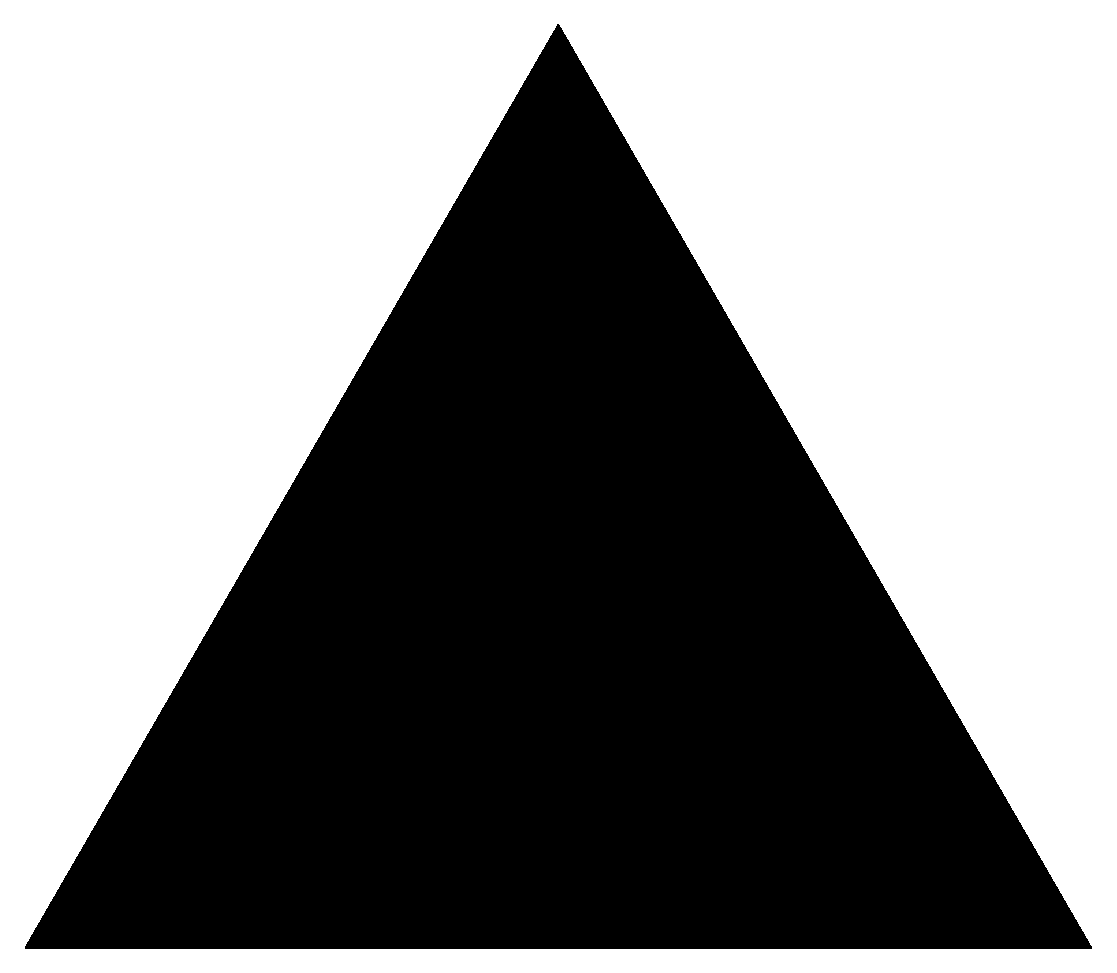
\includegraphics[width=\textwidth]{sierpinsky-triangle-iter0.pdf}
        \begin{center}
            $n=0$
        \end{center}
    \end{subfigure}
    \qquad
    \vspace{1cm}
    \begin{subfigure}{0.45\textwidth}
        \centering
        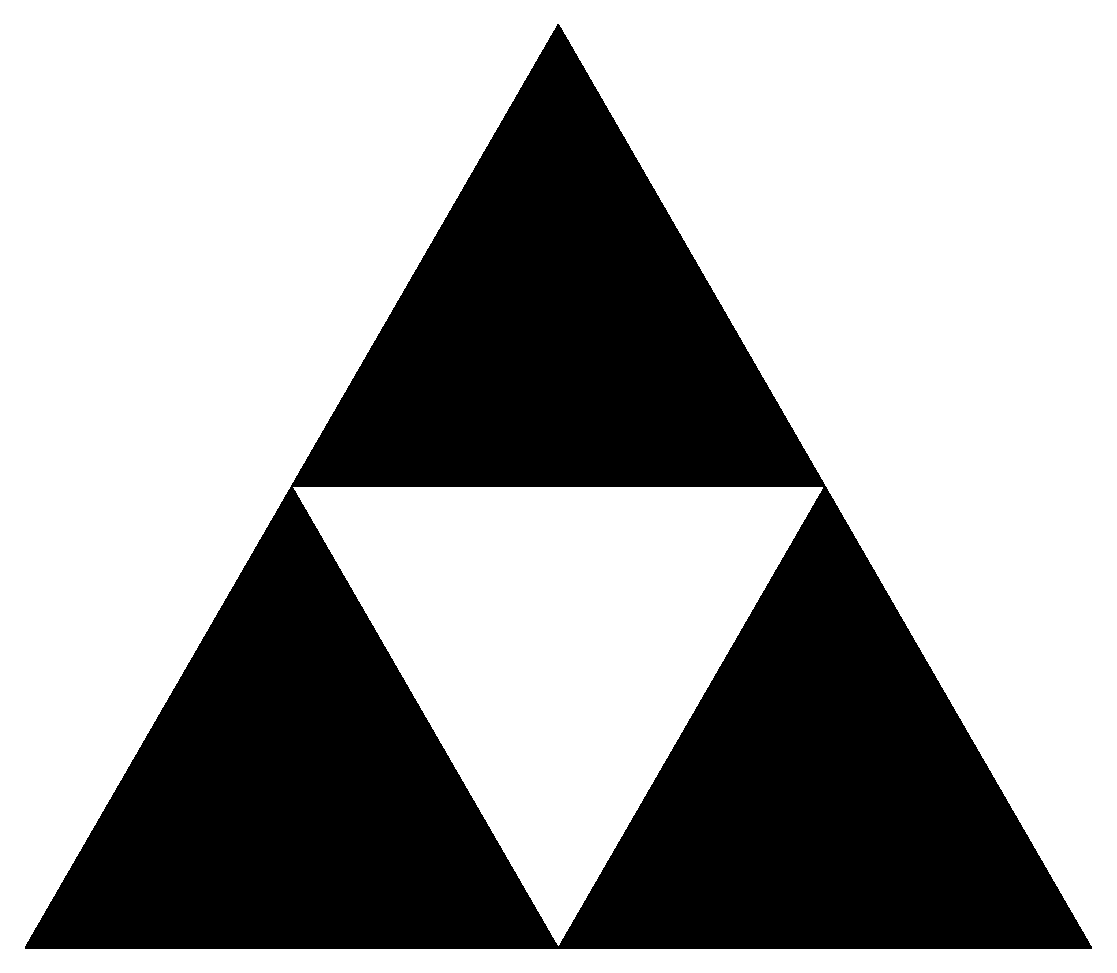
\includegraphics[width=\textwidth]{sierpinsky-triangle-iter1.pdf}
        \begin{center}
            $n=1$
        \end{center}
    \end{subfigure}
    \qquad
    \begin{subfigure}{0.45\textwidth}
        \centering
        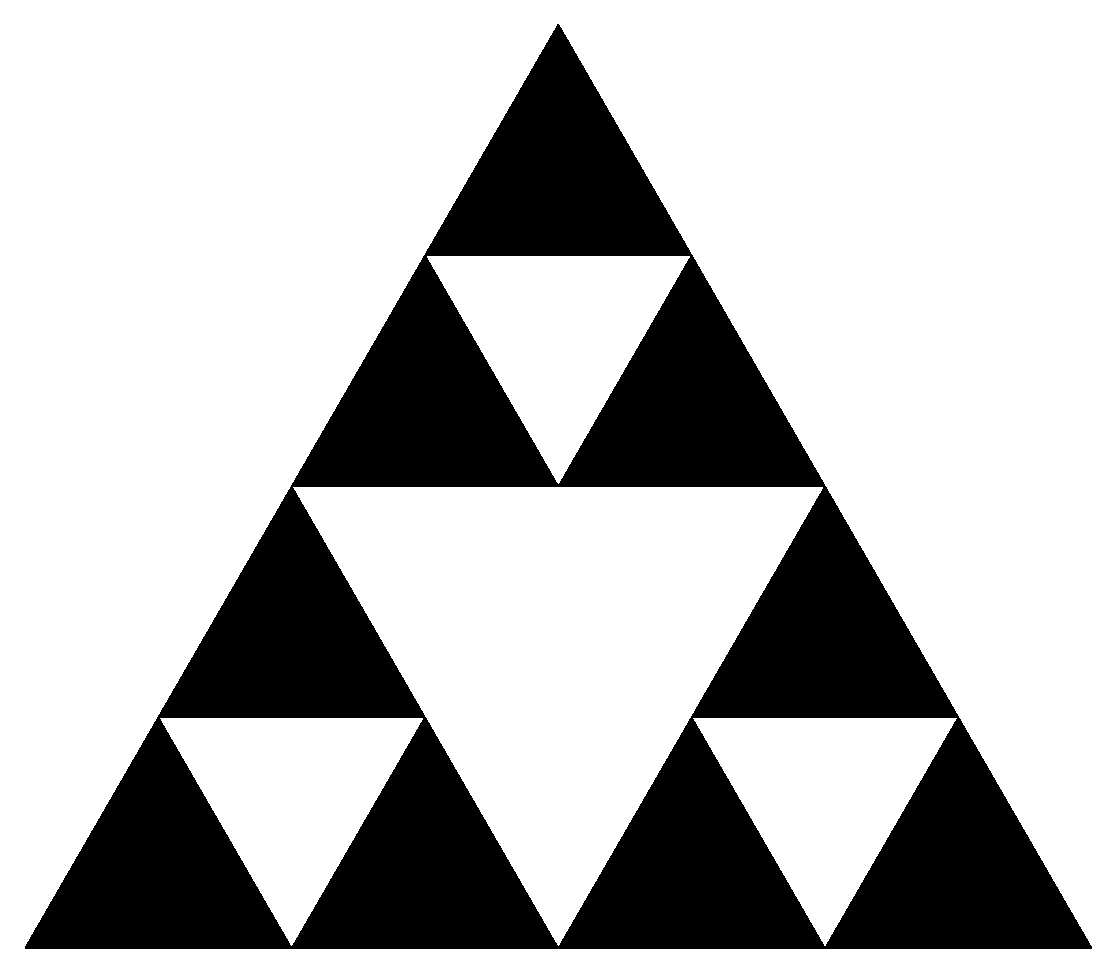
\includegraphics[width=\textwidth]{sierpinsky-triangle-iter2.pdf}
        \begin{center}
            $n=2$
        \end{center}
    \end{subfigure}
    \qquad
    \vspace{1cm}
    \begin{subfigure}{0.45\textwidth}
        \centering
        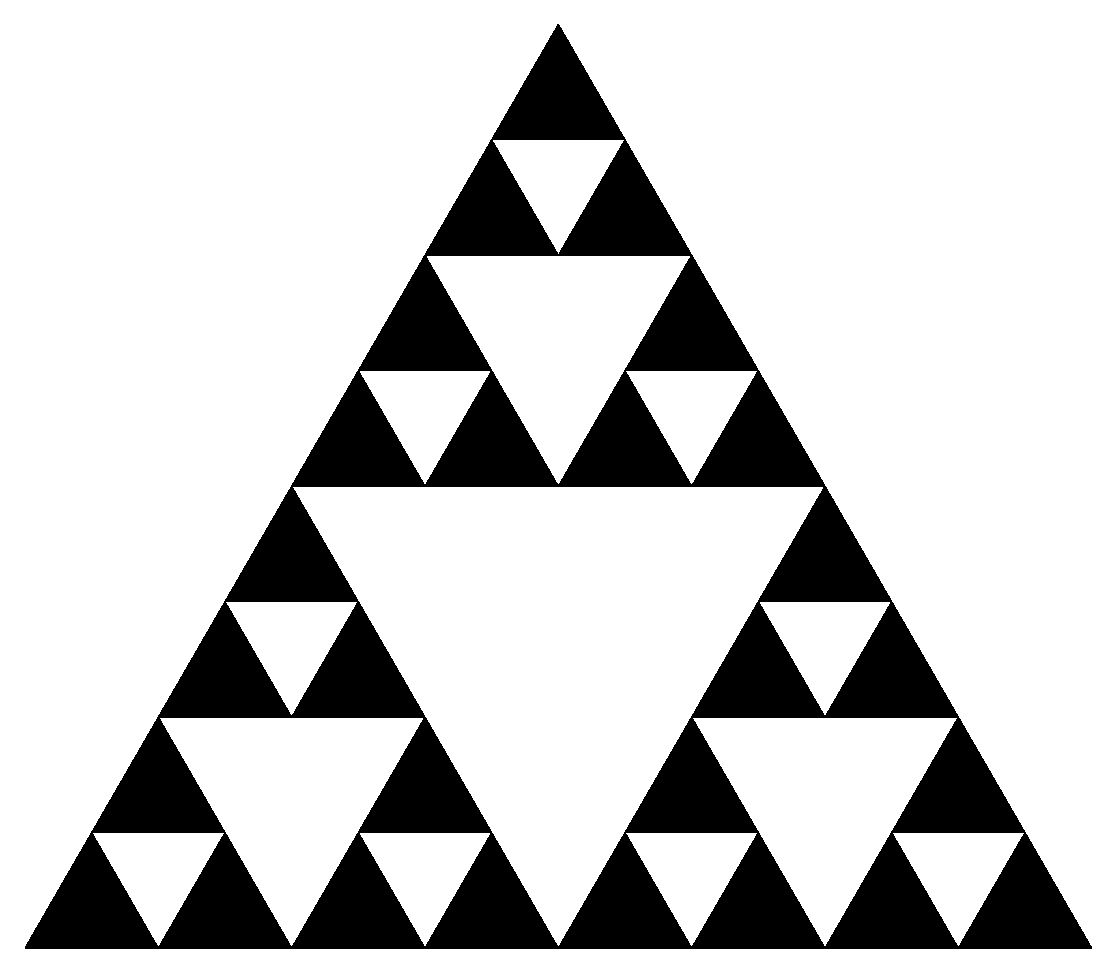
\includegraphics[width=\textwidth]{sierpinsky-triangle-iter3.pdf}
        \begin{center}
            $n=3$
        \end{center}
    \end{subfigure}
    \qquad
    \begin{subfigure}{0.45\textwidth}
        \centering
        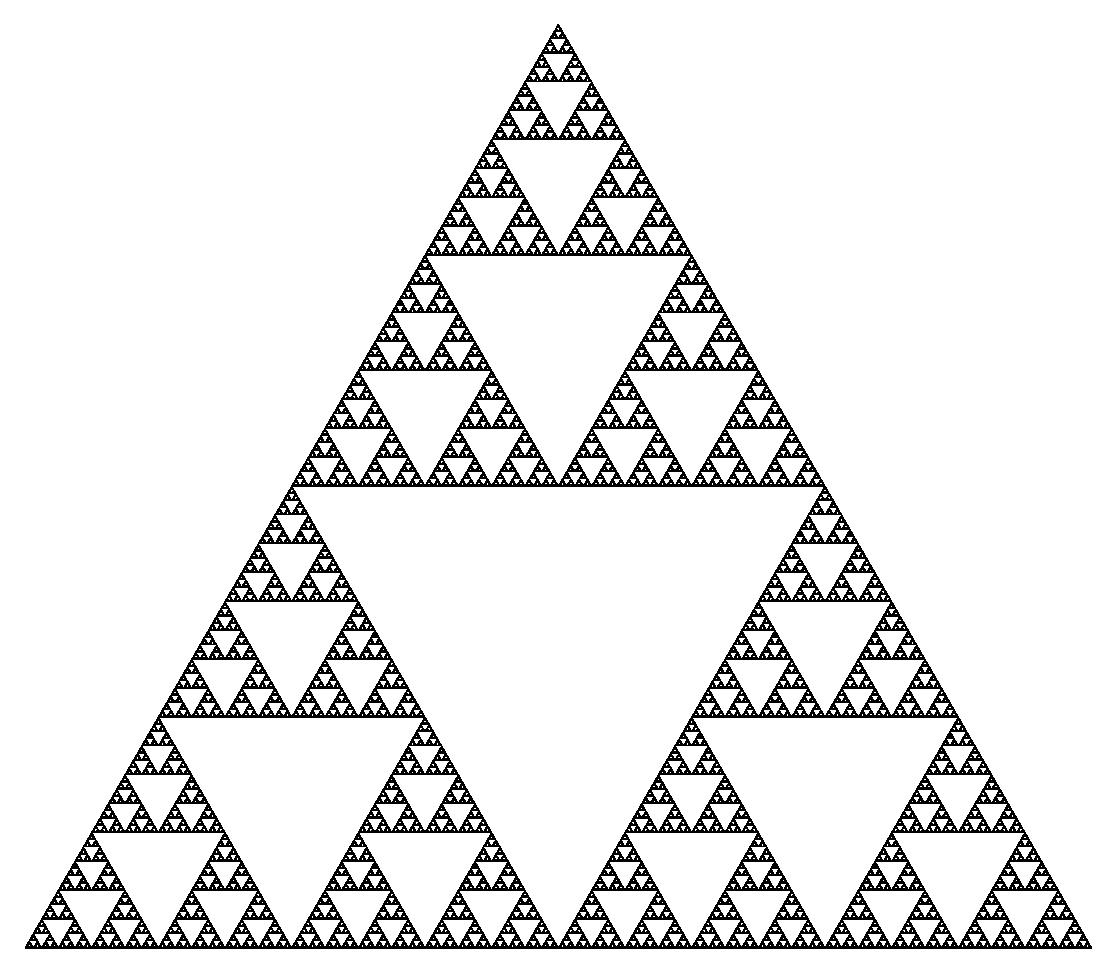
\includegraphics[width=\textwidth]{sierpinsky-triangle-iter8.pdf}
        \begin{center}
            $n=8$
        \end{center}
    \end{subfigure}
    \caption{Iterace zobrazení $\Omega$  (Sierpińského trojúhelník)}
    \label{fig:iterace-zobrazeni-omega-sierpinskeho-trojuhelnik}
\end{figure}
\clearpage
\begin{figure}[H]
    \centering
    \begin{subfigure}{0.45\textwidth}
        \centering
        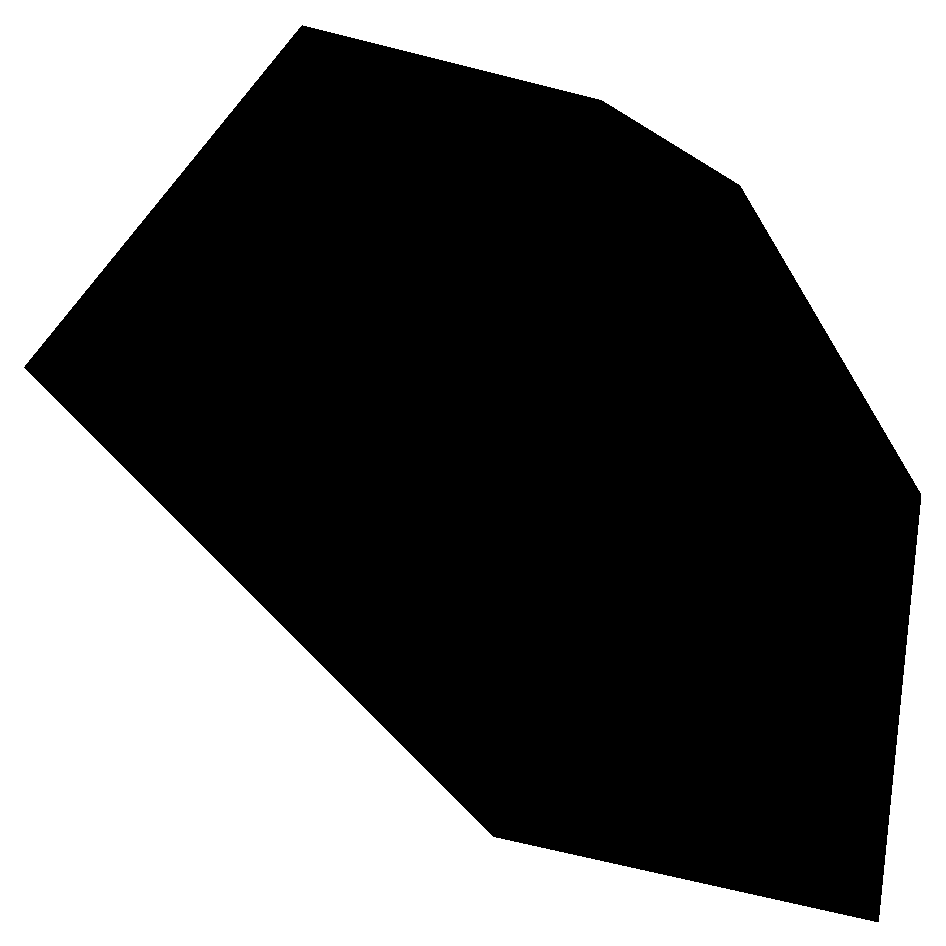
\includegraphics[width=\textwidth]{sierpinsky-triangle-2-iter0.pdf}
        \begin{center}
            $n=0$
        \end{center}
    \end{subfigure}
    \qquad
    \vspace{1cm}
    \begin{subfigure}{0.45\textwidth}
        \centering
        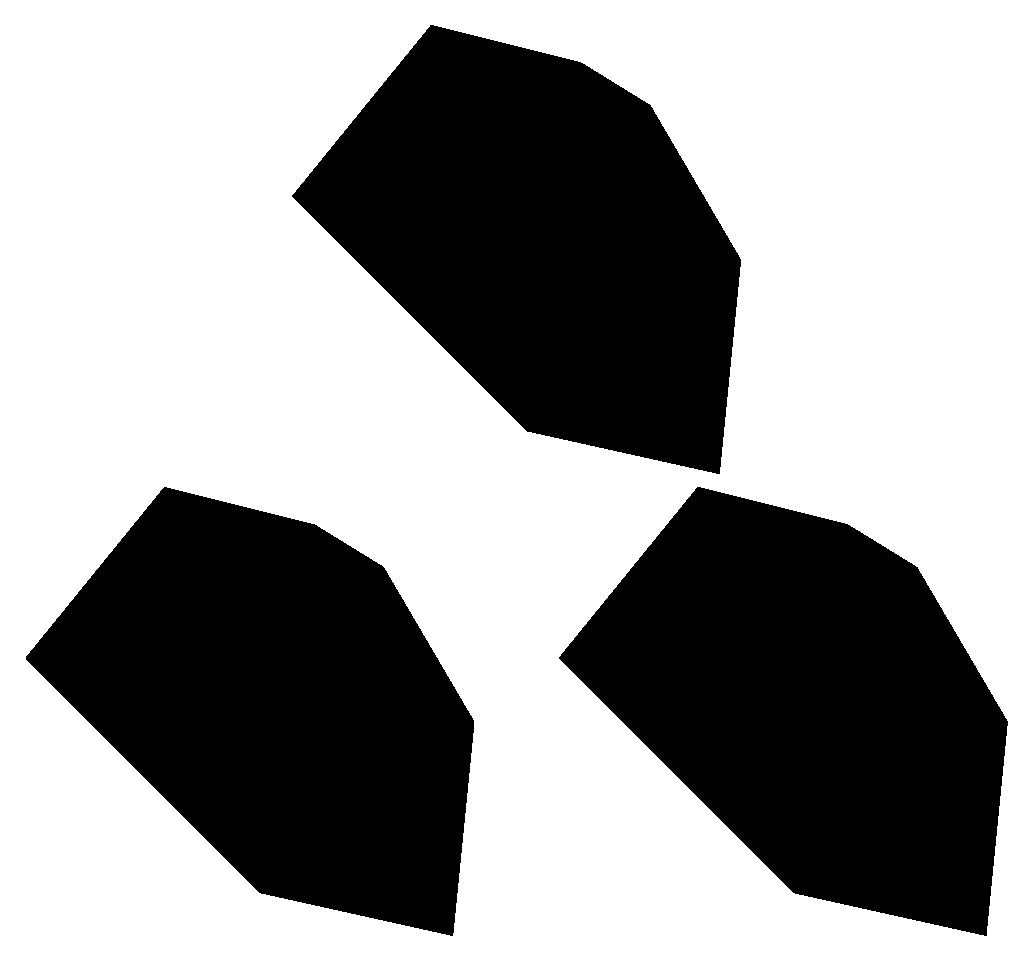
\includegraphics[width=\textwidth]{sierpinsky-triangle-2-iter1.pdf}
        \begin{center}
            $n=1$
        \end{center}
    \end{subfigure}
    \qquad
    \begin{subfigure}{0.45\textwidth}
        \centering
        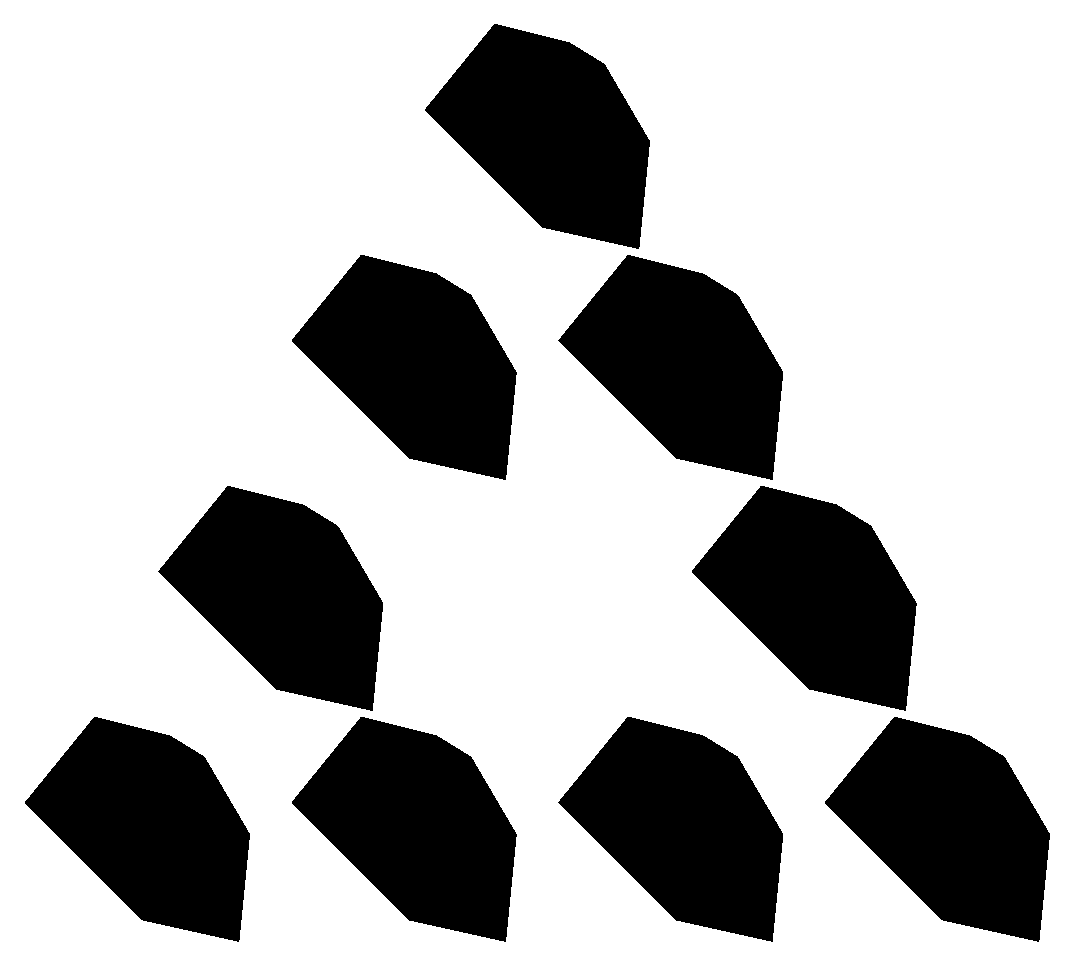
\includegraphics[width=\textwidth]{sierpinsky-triangle-2-iter2.pdf}
        \begin{center}
            $n=2$
        \end{center}
    \end{subfigure}
    \qquad
    \vspace{1cm}
    \begin{subfigure}{0.45\textwidth}
        \centering
        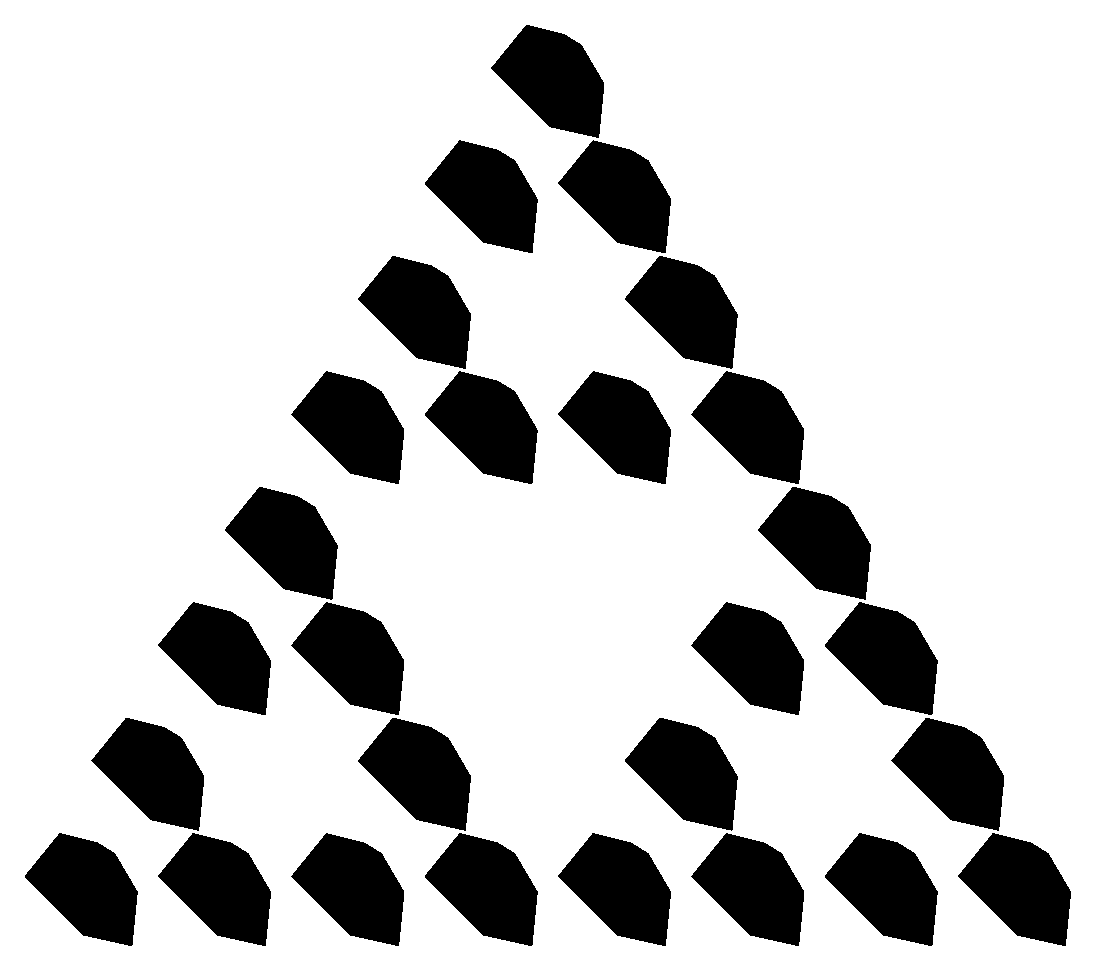
\includegraphics[width=\textwidth]{sierpinsky-triangle-2-iter3.pdf}
        \begin{center}
            $n=3$
        \end{center}
    \end{subfigure}
    \qquad
    \begin{subfigure}{0.45\textwidth}
        \centering
        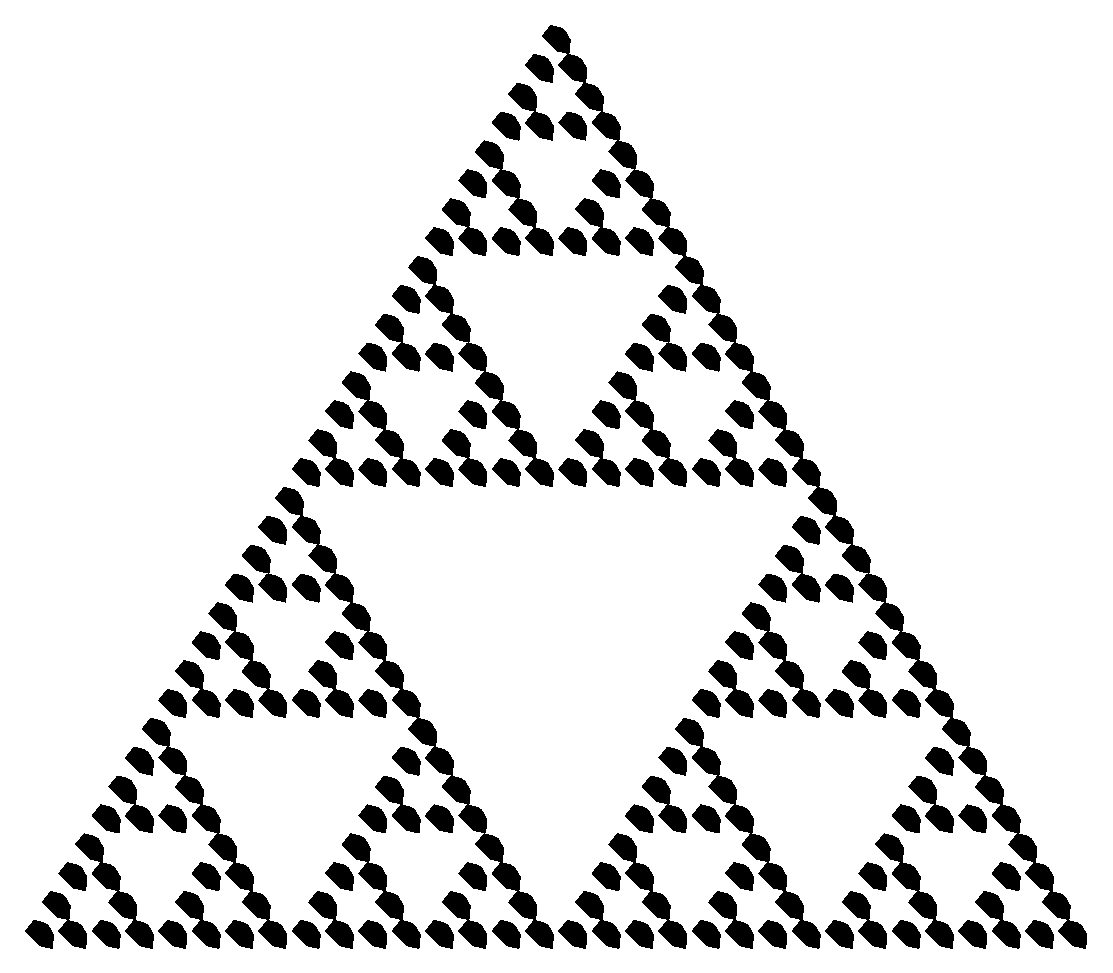
\includegraphics[width=\textwidth]{sierpinsky-triangle-2-iter5.pdf}
        \begin{center}
            $n=5$
        \end{center}
    \end{subfigure}
    \qquad
    \begin{subfigure}{0.45\textwidth}
        \centering
        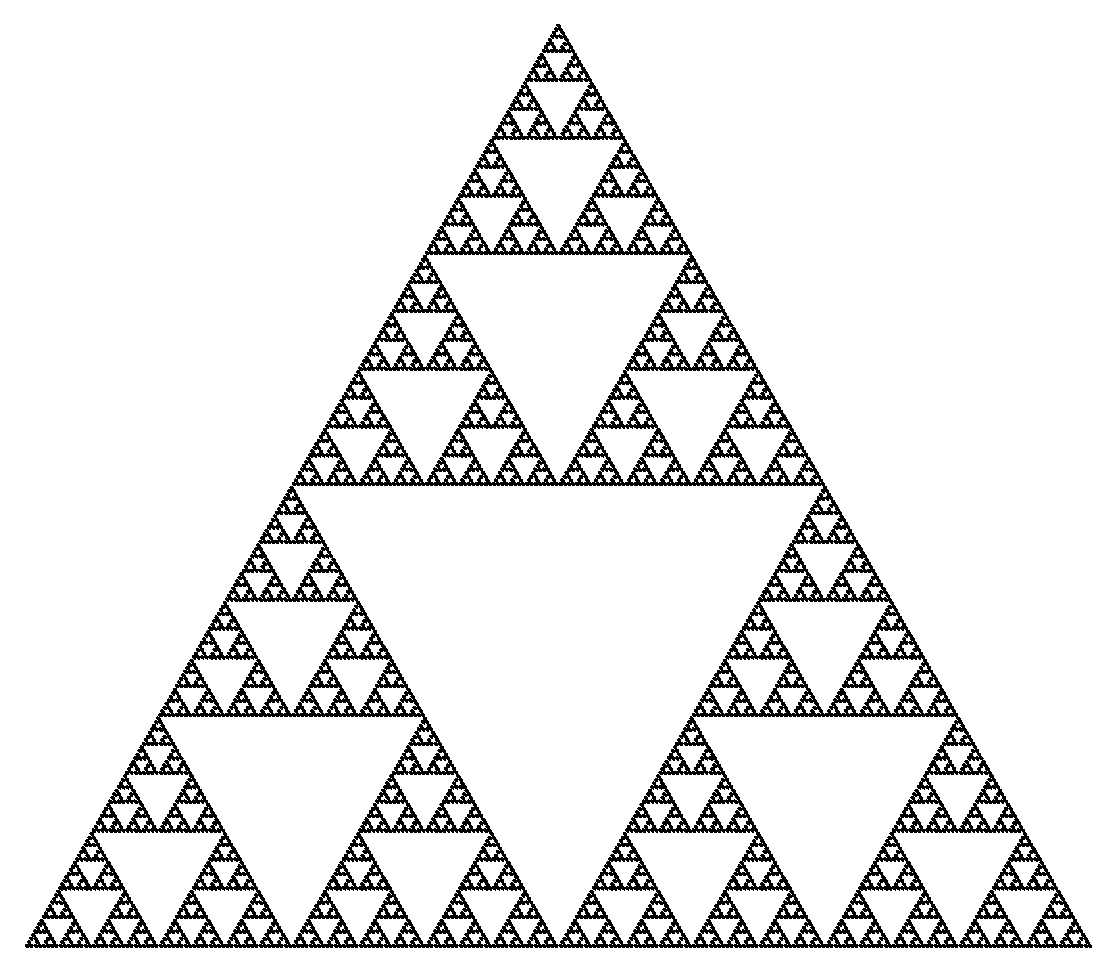
\includegraphics[width=\textwidth]{sierpinsky-triangle-2-iter8.pdf}
        \begin{center}
            $n=8$
        \end{center}
    \end{subfigure}
    \caption{Iterace zobrazení $\Omega$ s~jiným počátečním útvarem $B$}
    \label{fig:iterace-zobrazeni-omega-sierpinskeho-trojuhelnik-jiny-poc-utvar}
\end{figure}
\begin{figure}[H]
    \centering
    \begin{subfigure}{0.45\textwidth}
        \centering
        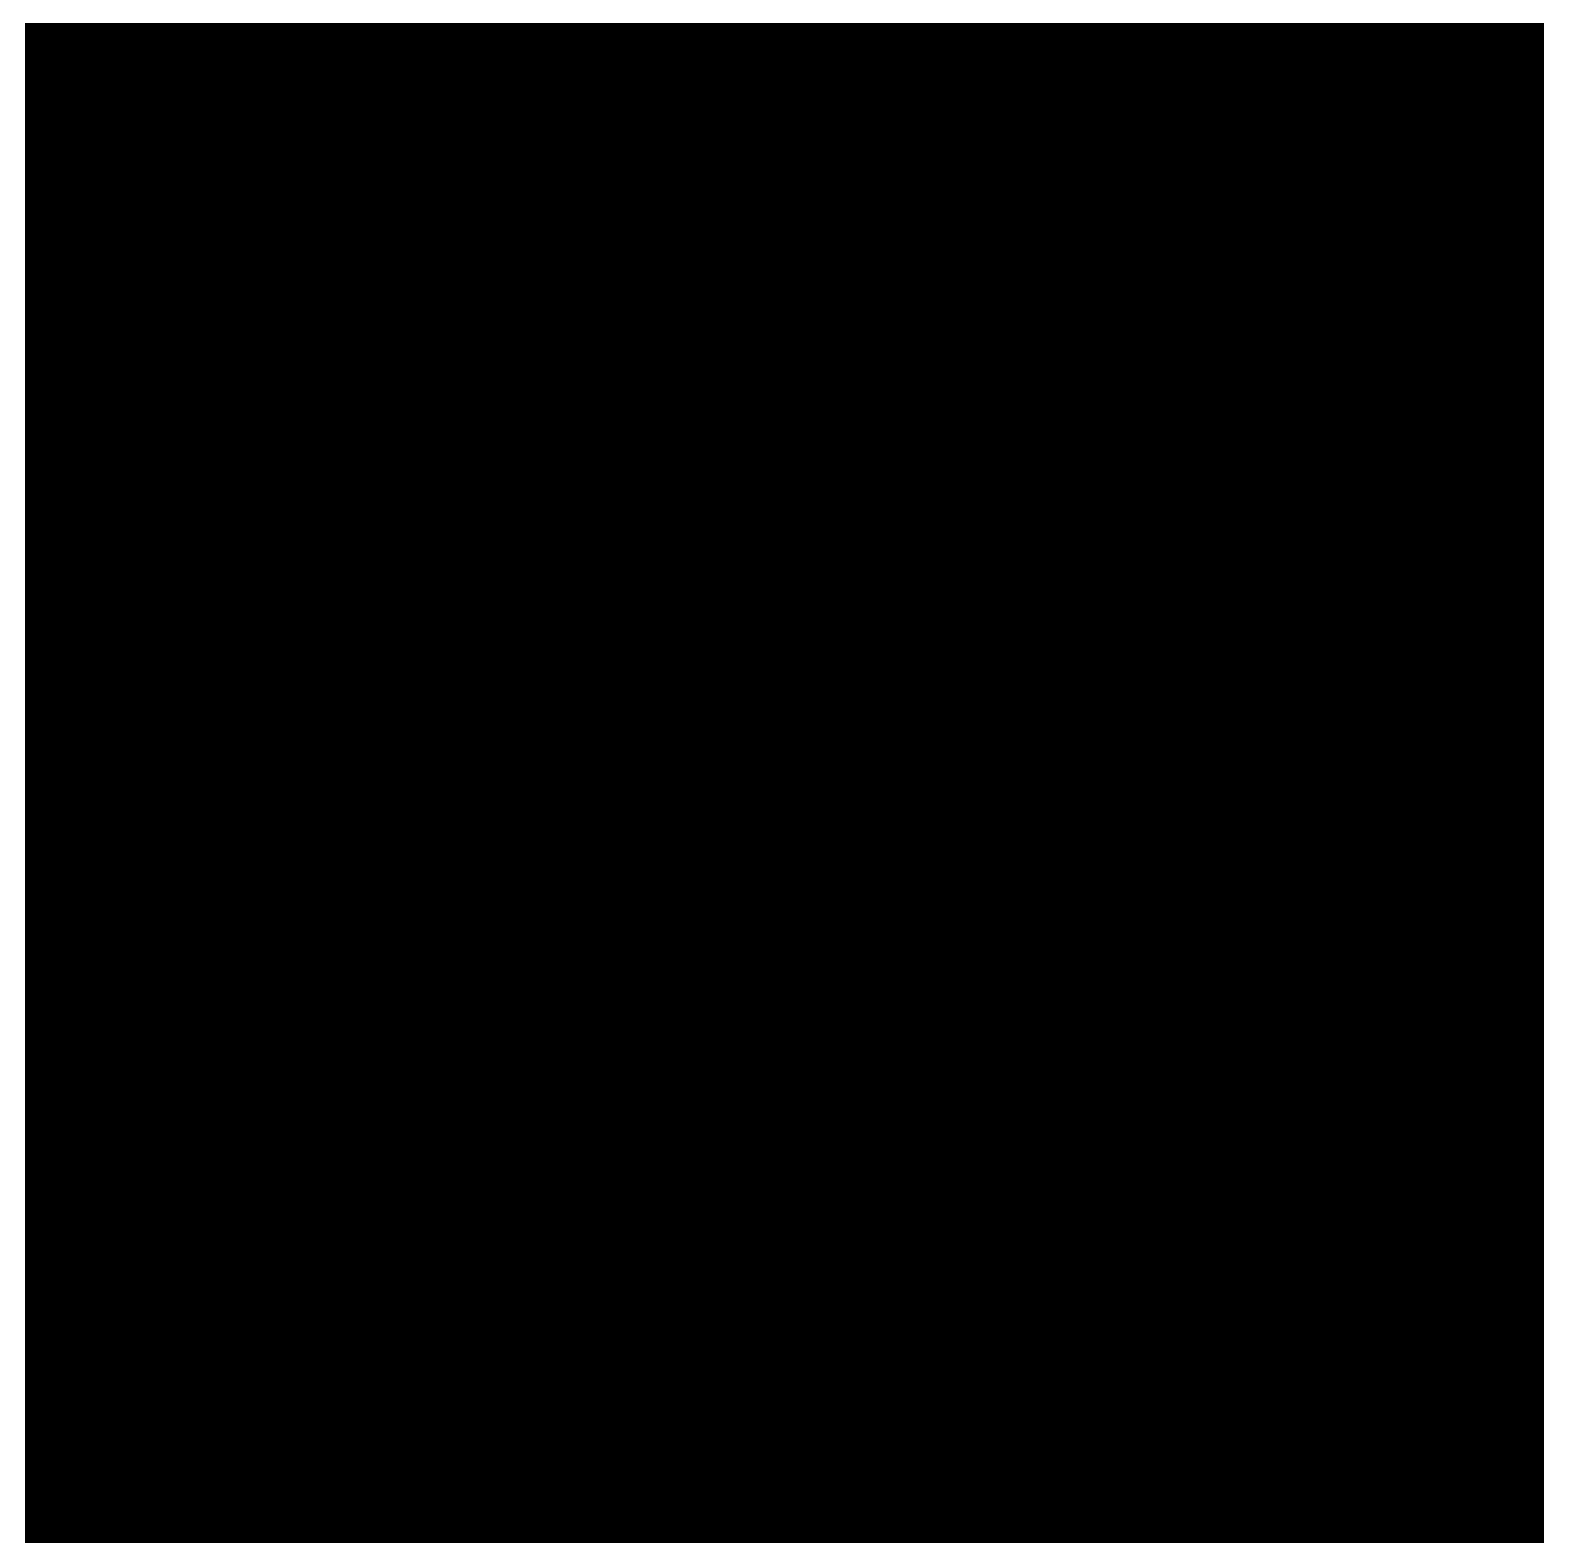
\includegraphics[width=\textwidth]{sierpinsky-carpet-iter0.pdf}
        \begin{center}
            $n=0$
        \end{center}
    \end{subfigure}
    \qquad
    \vspace{1cm}
    \begin{subfigure}{0.45\textwidth}
        \centering
        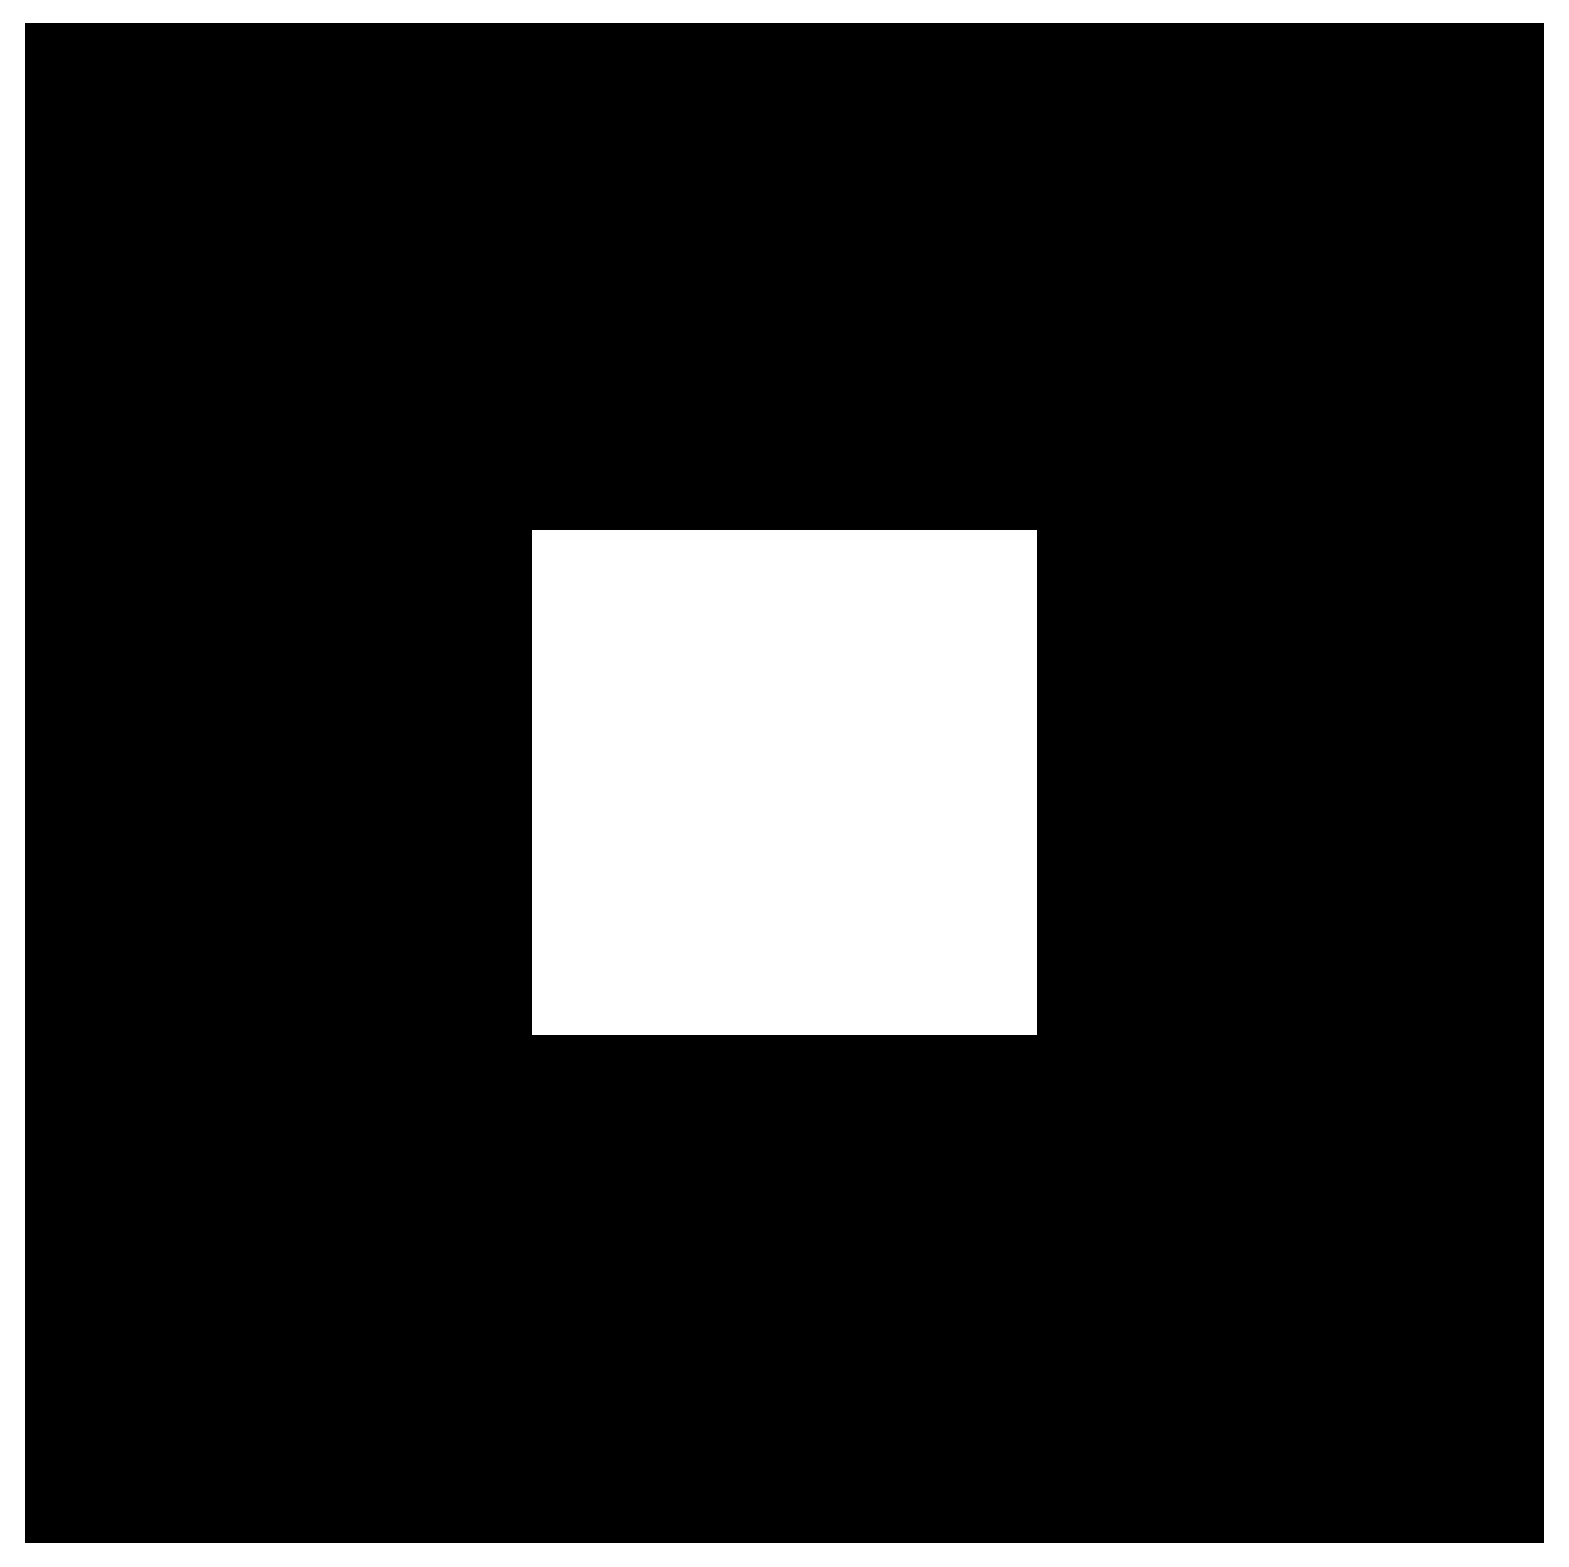
\includegraphics[width=\textwidth]{sierpinsky-carpet-iter1.pdf}
        \begin{center}
            $n=1$
        \end{center}
    \end{subfigure}
    \qquad
    \begin{subfigure}{0.45\textwidth}
        \centering
        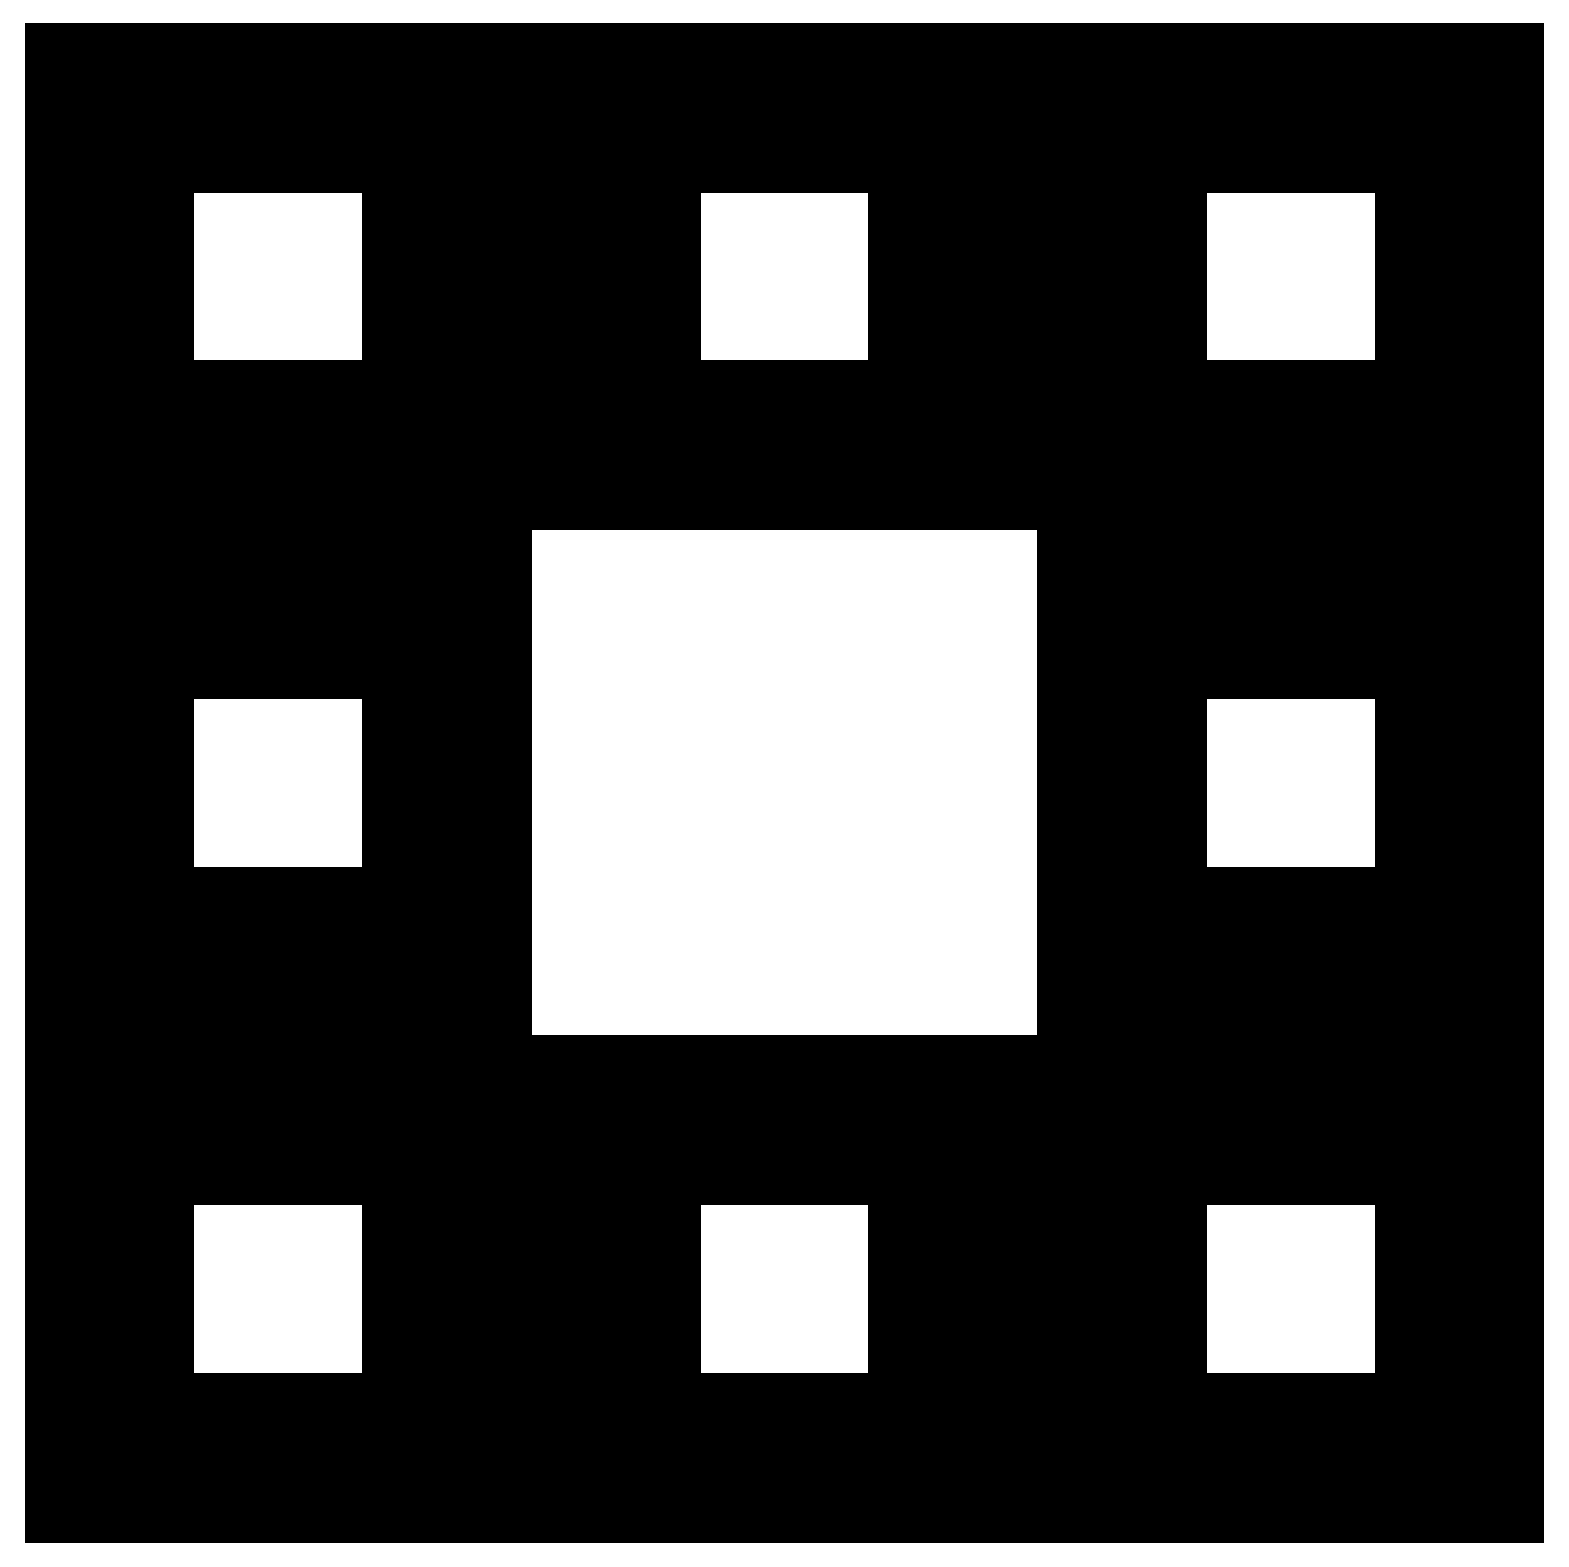
\includegraphics[width=\textwidth]{sierpinsky-carpet-iter2.pdf}
        \begin{center}
            $n=2$
        \end{center}
    \end{subfigure}
    \qquad
    \vspace{1cm}
    \begin{subfigure}{0.45\textwidth}
        \centering
        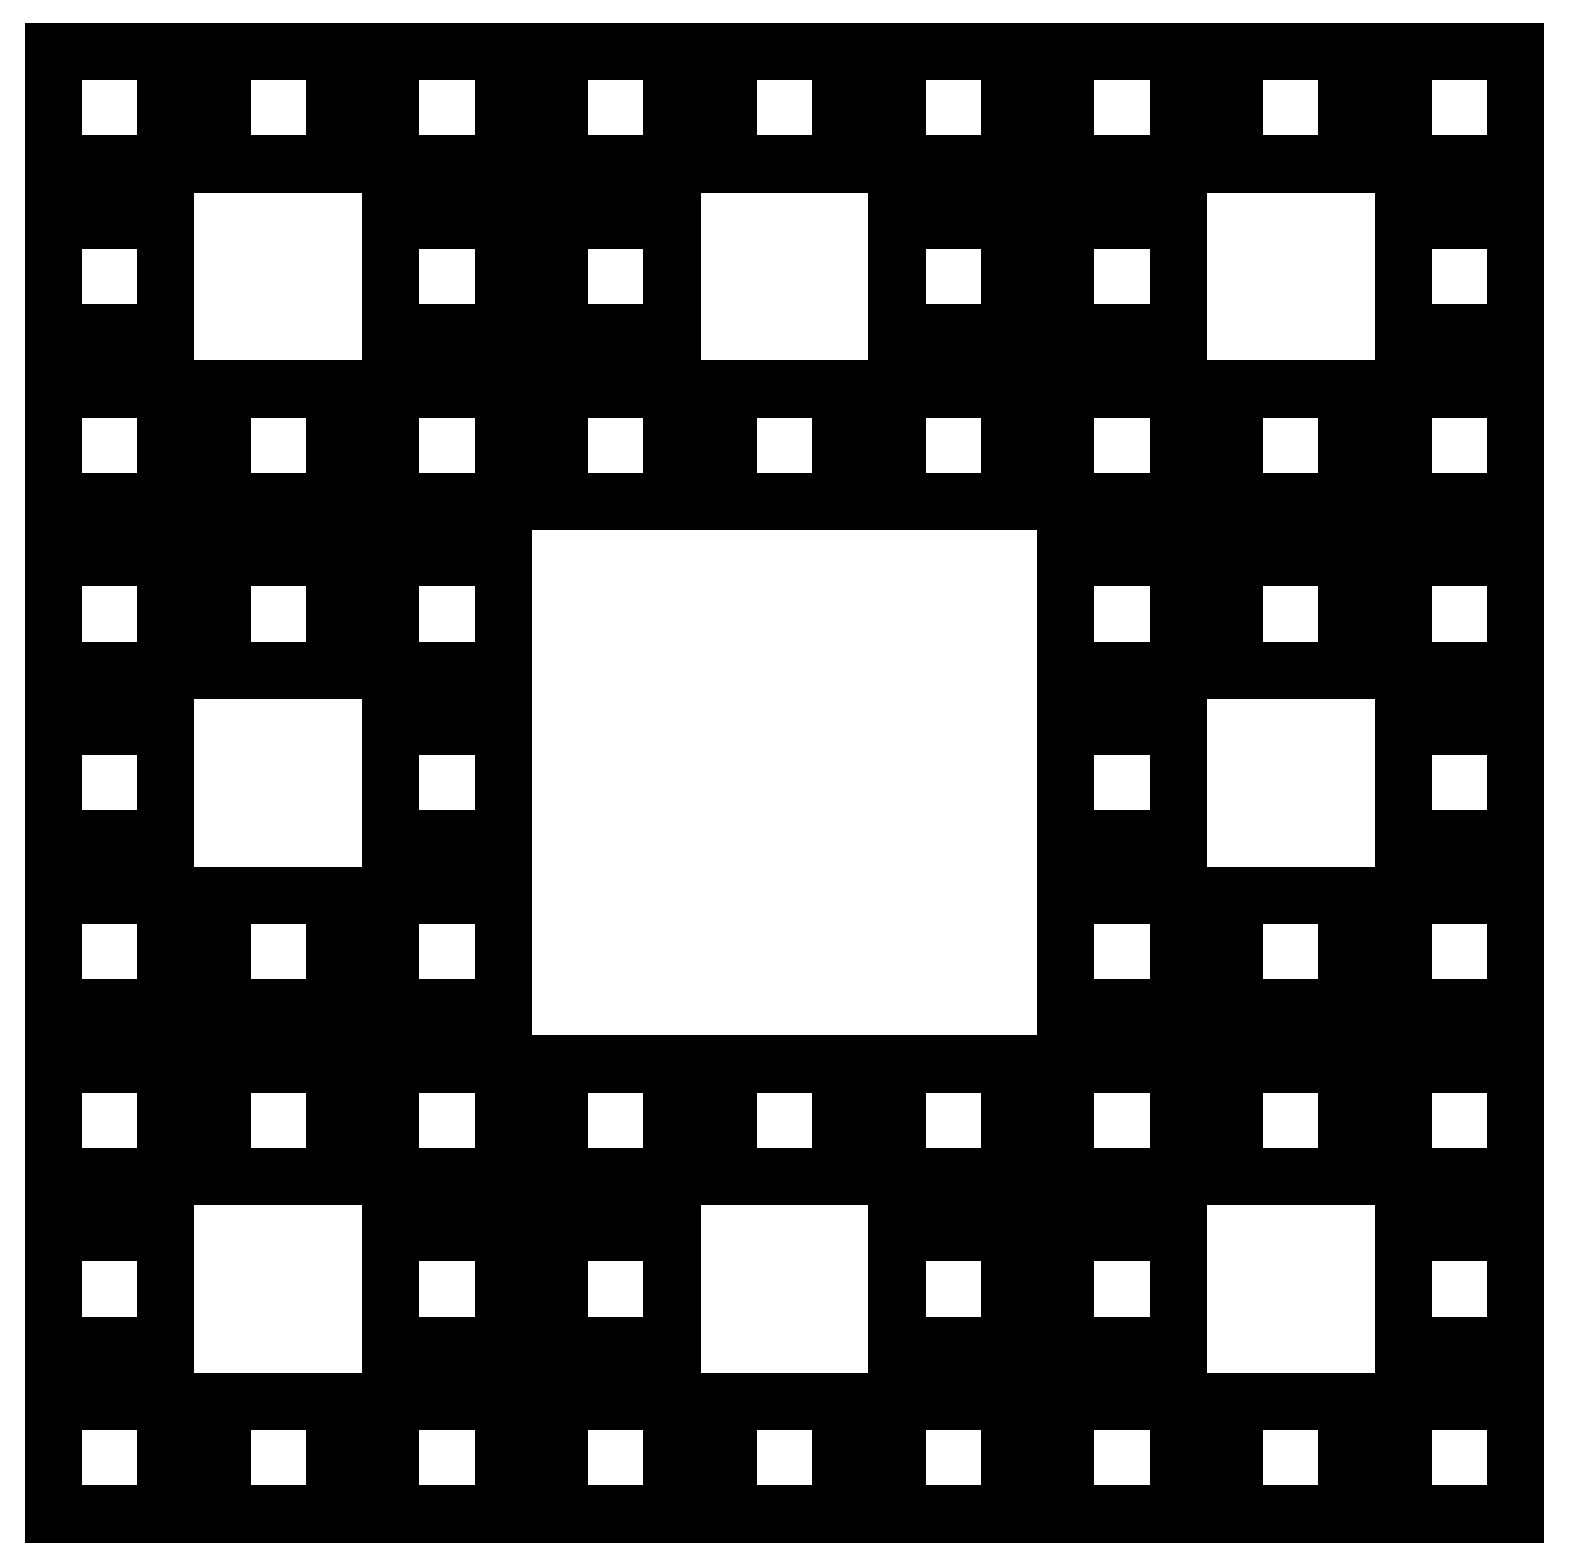
\includegraphics[width=\textwidth]{sierpinsky-carpet-iter3.pdf}
        \begin{center}
            $n=3$
        \end{center}
    \end{subfigure}
    \qquad
    \begin{subfigure}{0.45\textwidth}
        \centering
        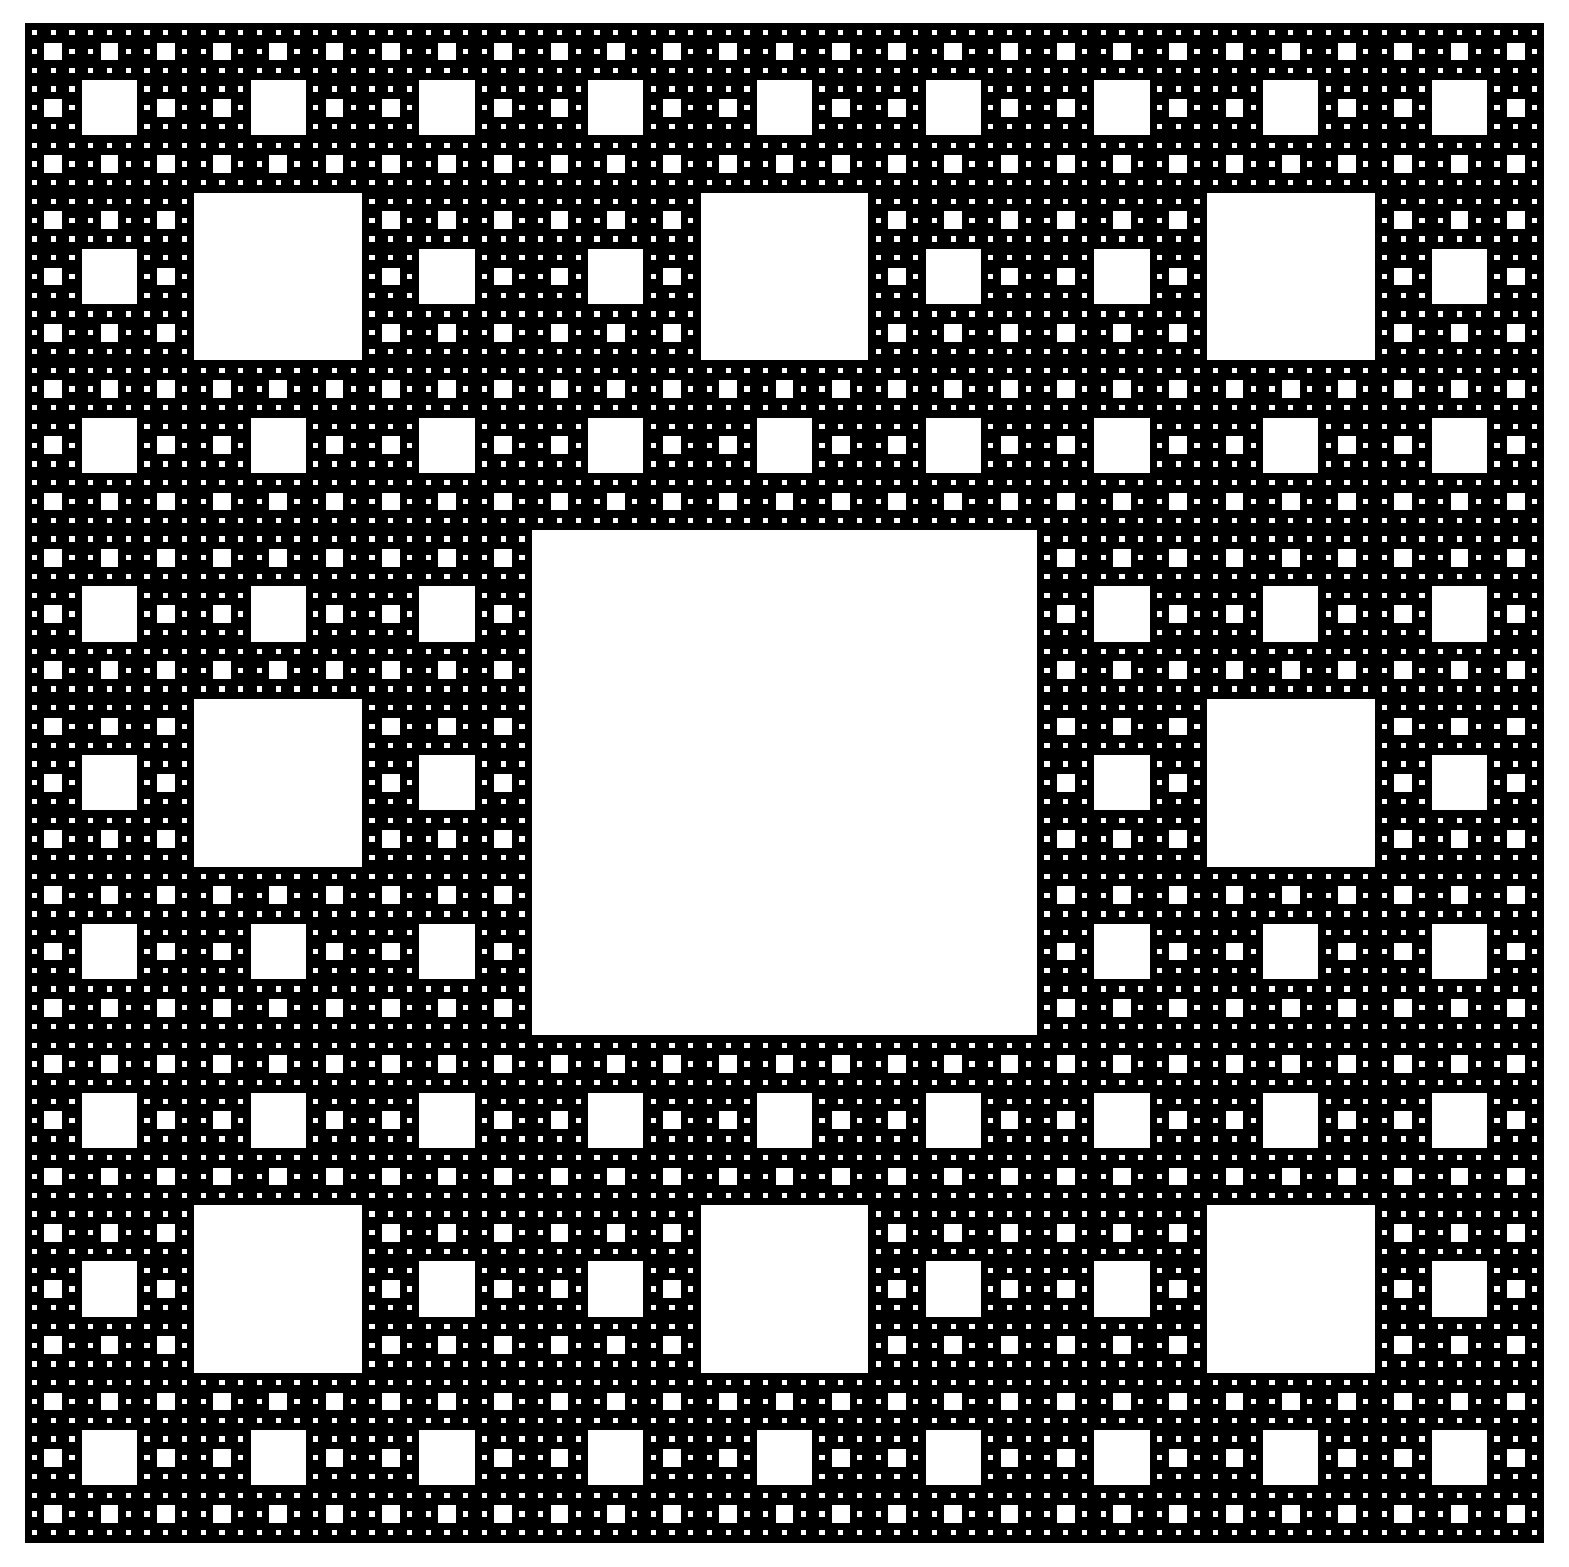
\includegraphics[width=\textwidth]{sierpinsky-carpet-iter5.pdf}
        \begin{center}
            $n=5$
        \end{center}
    \end{subfigure}
    \caption{Iterace zobrazení $\Phi$ (Sierpińského koberec)}
    \label{fig:iterace-zobrazeni-fi-sierpinskeho-koberec}
\end{figure}

\subsection{Další fraktály a~jejich IFS}\label{subsec:fraktaly-a-jejich-ifs}

V této podsekci se podíváme na některé další příklady fraktálů a~jejich IFS. I~zde jsou všechny obrázky vygenerovány pomocí přiloženého programu\footnote{viz odkaz na GitHub repozitář: \url{https://github.com/D4vEOFF/Py-Fractal-Generator}}.
\begin{figure}[H]
    \centering
    \includegraphics[width=0.8\textwidth]{pythagorean-tree-iter10.pdf}
    \begin{center}
        $n=10$
    \end{center}
    \begin{tabular}{c|cccccc}
    Zobrazení   & $a$   & $b$   & $c$   & $d$   & $e$   & $f$          \\\hline
    $\psi_1$    & $1/2$ & $-1/2$ & $1/2$ & $1/2$ & $0$   & $1$         \\
    $\psi_2$    & $1/2$ & $1/2$ & $-1/2$ & $1/2$ & $1/2$ & $3/2$         \\
    $\psi_3$    & $1$   & $0$   & $0$   & $1$   & $0$   & $0$         \\
    \end{tabular}
    \caption{Pythágorův strom}
    \label{fig:pythagoruv-strom}
\end{figure}
Zde upozorněme však na fakt, že u~Pythágorova stromu na obrázku~\ref{fig:pythagoruv-strom} zobrazení $\psi_3$ je identita, která není kontrakcí, čili na takový systém nelze aplikovat větu~\ref{thm:sjednoceni-kontrakci}. Toto zobrazení je zde však čistě z~estetických důvodů, aby původní obrazec nezměnil svoji pozici v~další iteraci. Systém $\set{\psi_1,\psi_2}$ již představuje IFS s~jednoznačným atraktorem.
\begin{figure}[H]
    \centering
    \includegraphics[width=0.8\textwidth]{levi-dragon-iter12.pdf}
    \begin{center}
        $n=12$
    \end{center}
    \begin{tabular}{c|cccccc}
    Kontrakce   & $a$   & $b$   & $c$   & $d$   & $e$   & $f$          \\\hline
    $\psi_1$    & $1/2$ & $-1/2$ & $1/2$ & $1/2$ & $0$   & $0$         \\
    $\psi_2$    & $1/2$ & $1/2$ & $-1/2$ & $1/2$ & $1/2$ & $1/2$
    \end{tabular}
    \caption{Lévyho drak}
    \label{fig:levyho-drak}
\end{figure}
\begin{figure}[H]
    \centering
    \includegraphics[width=0.8\textwidth]{heighway-dragon-iter15.pdf}
    \begin{center}
        $n=15$
    \end{center}
    \begin{tabular}{c|cccccc}
    Kontrakce   & $a$   & $b$   & $c$   & $d$   & $e$   & $f$          \\\hline
    $\psi_1$    & $1/2$ & $-1/2$ & $1/2$ & $1/2$ & $0$   & $0$         \\
    $\psi_2$    & $-1/2$ & $-1/2$ & $1/2$ & $-1/2$ & $1$ & $0$
    \end{tabular}
    \caption{Dračí křivka}
    \label{fig:draci-krivka}
\end{figure}
\begin{figure}[H]
    \centering
    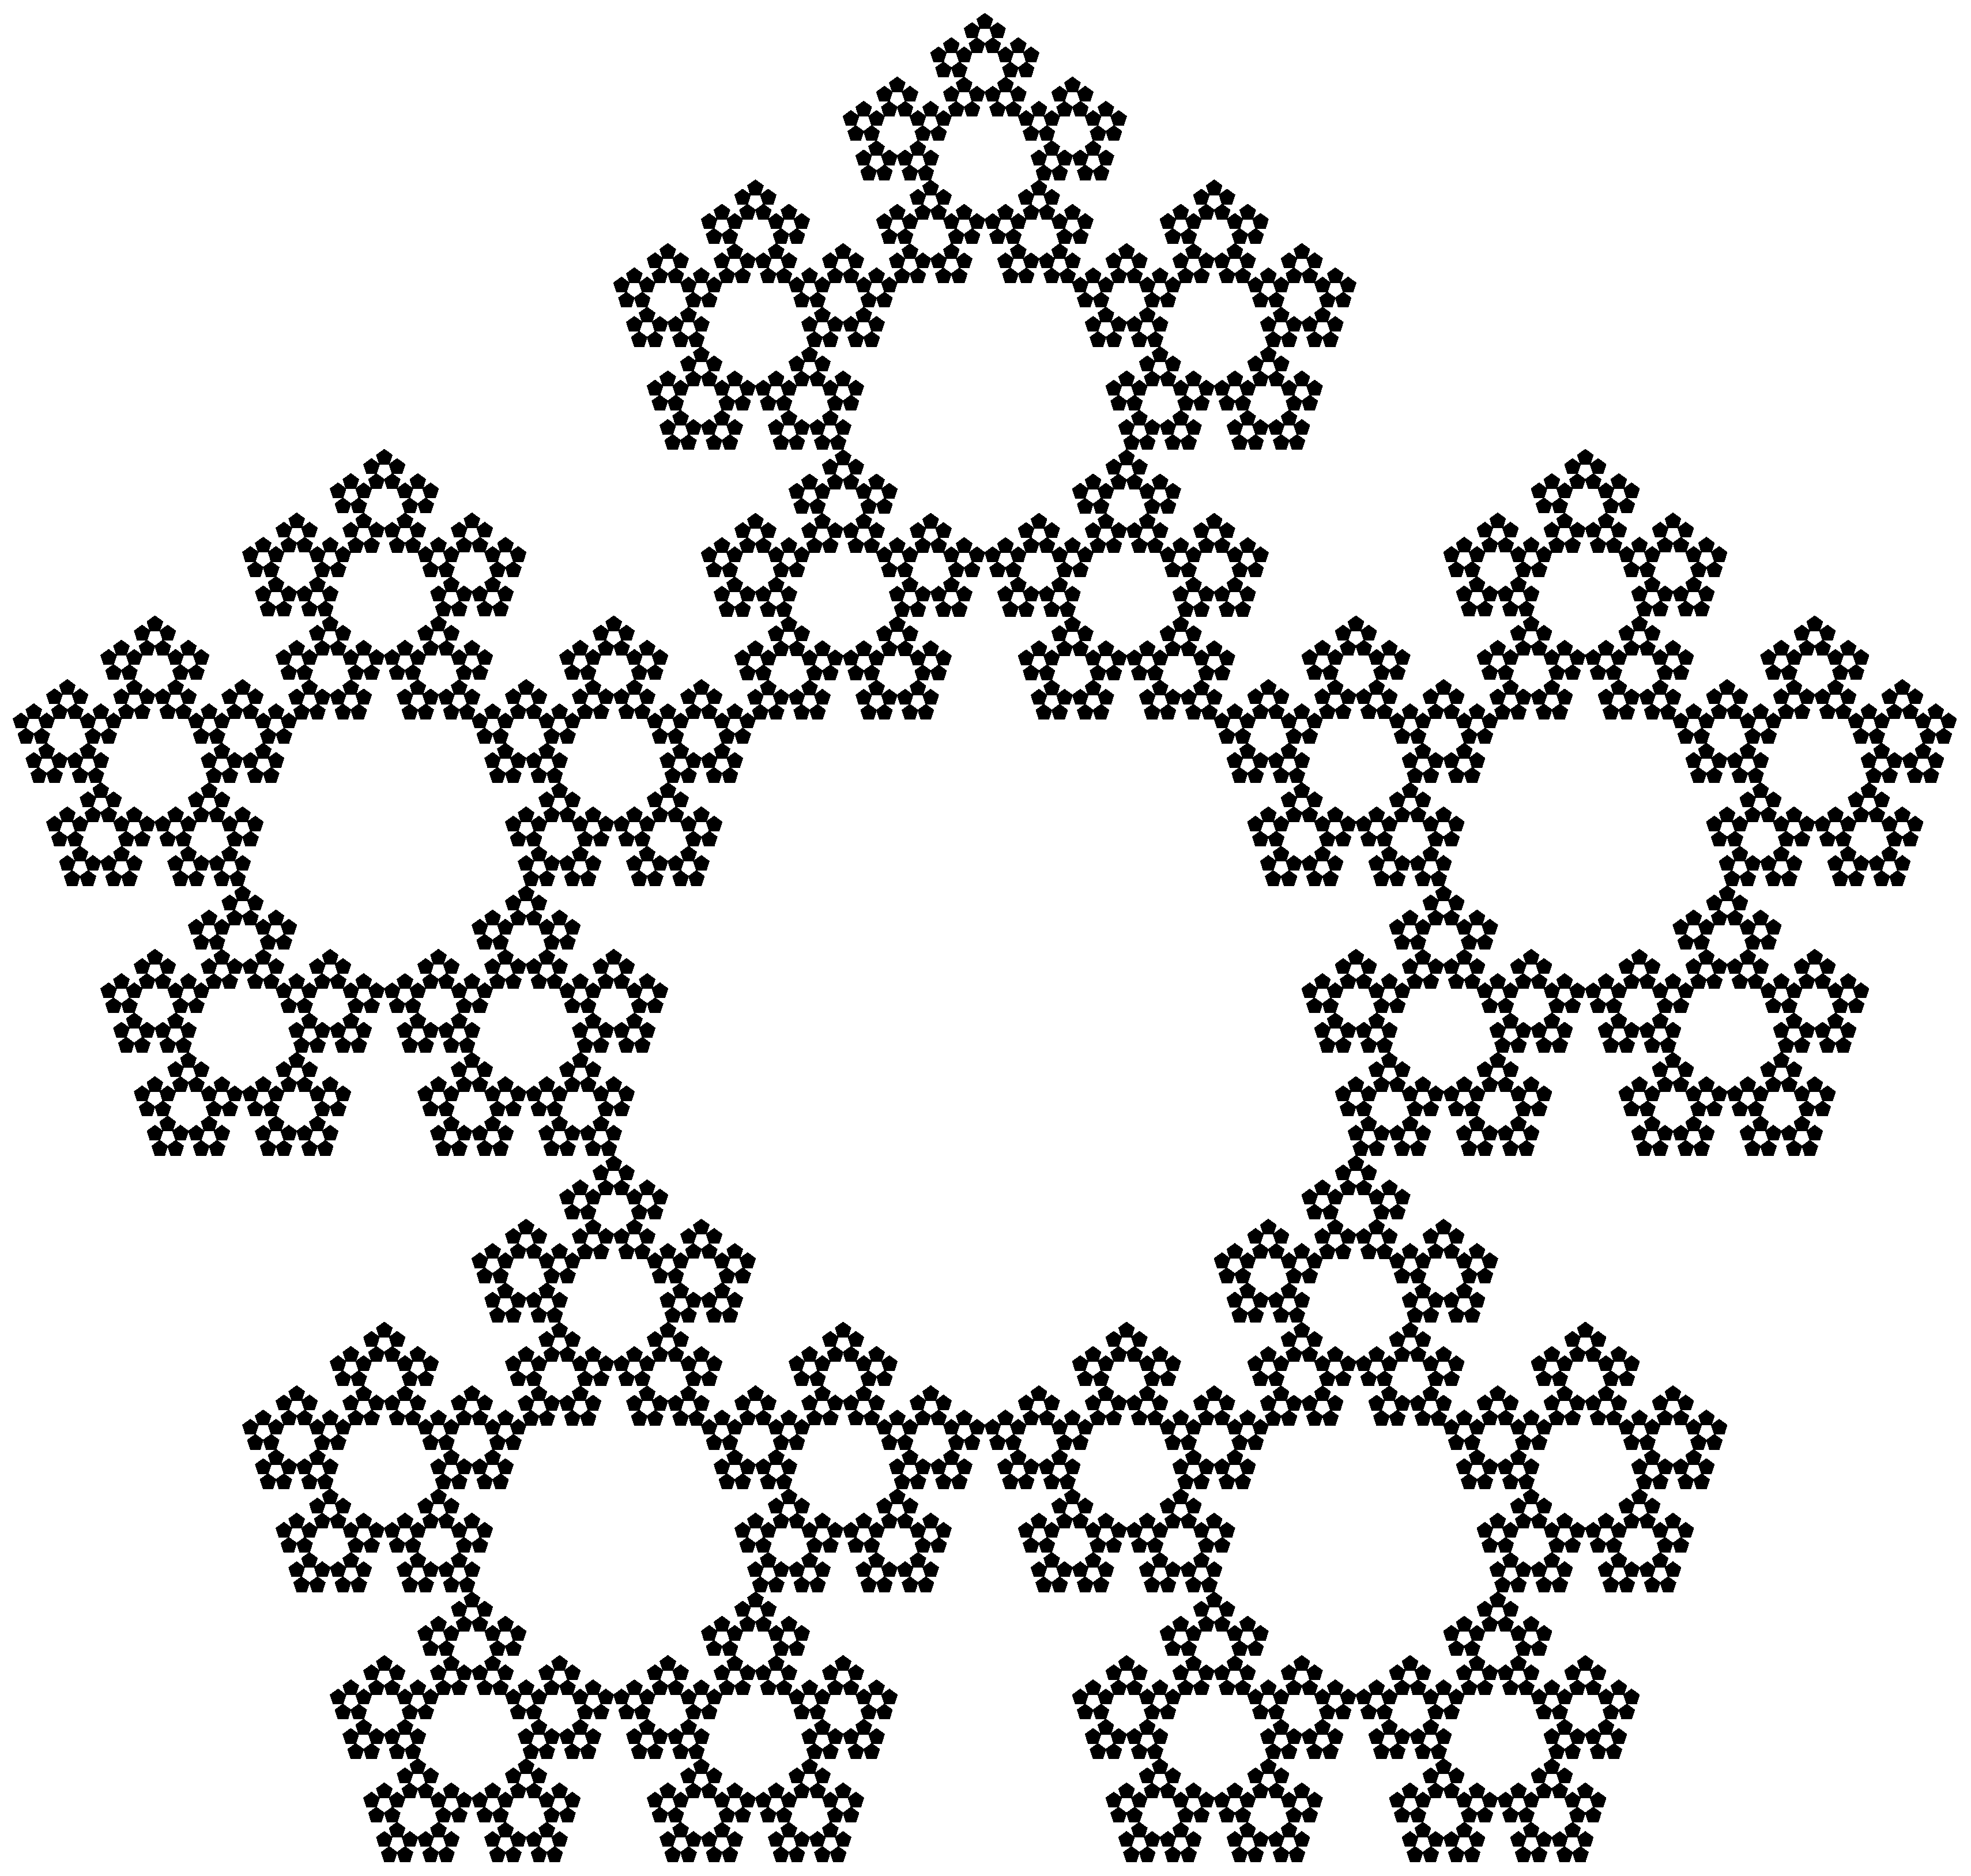
\includegraphics[width=0.8\textwidth]{sierpinsky-pentagon-iter5.pdf}
    \begin{center}
        $n=5$
    \end{center}
    \begin{tabular}{c|cccccc}
    Kontrakce   & $a$   & $b$   & $c$   & $d$   & $e$   & $f$                   \\\hline
    $\psi_1$    & $0{,}382$ & $0$ & $0$ & $0{,}382$ & $0$   & $0$               \\
    $\psi_2$    & $0{,}382$ & $0$ & $0$ & $0{,}382$ & $0{,}618$   & $0$         \\
    $\psi_3$    & $0{,}382$ & $0$ & $0$ & $0{,}382$ & $0{,}809$   & $0{,}588$   \\
    $\psi_4$    & $0{,}382$ & $0$ & $0$ & $0{,}382$ & $0{,}309$   & $0{,}951$   \\
    $\psi_5$    & $0{,}382$ & $0$ & $0$ & $0{,}382$ & $-0{,}191$   & $0{,}588$  \\
    \end{tabular}
    \caption{Sierpińského pětiúhelník}
    \label{fig:sierpinskeho-petiuhelnik}
\end{figure}

\subsection{IFS a~výpočet dimenze}\label{subsec:ifs-vypocet-dimenze}

Pojďme se ještě na chvíli vrátit k~tématu, které jsme již probírali v~úvodní kapitole~\ref{chapter:uvod_do_fraktalu} a~dále jsme se mu hlouběji věnovali v~kapitole~\ref{chapter:teorie-miry-a-dimenze} -- dimenzi. V~rámci tohoto textu jsme si ukázali dva základní typy, a to \emph{box-counting dimenzi}\index{dimenze!box-counting}\index{box-counting dimenze} a~\emph{Hausdorffovu dimenzi}\index{dimenze!Hausdorffova}\index{Hausdorffova dimenze}. V~této části navážeme na některé výsledky, k nimž jsme dospěli v~podsekcích~\ref{subsec:vlastnosti-hausdorffovy-miry} a~\ref{subsec:hausdorffova-dimenze}.

Ohlédněme se zpět za příkladem~\ref{ex:sierpinskeho-trojuhelnik-hd-dimenze}, kde jsme počítali Hausdorffovu dimenzi Sierpińského trojúhelníka celkově dvěma způsoby. První vycházel přímo z~její definice, zatímco druhý byl podstatně jednodušší, neboť pracoval s~netriviálním předpokladem, že míra daného útvaru je konečná. Z~onoho příkladu však nejspíše tušíme, že počítat Hausdorffovu dimenzi z~definice je dosti nepraktické. Proto si zkusíme druhý způsob výpočtu trochu přiblížit.

Než se však pustíme do dalšího výkladu, připomeňme si některé nám již známé výsledky. V~sekci~\ref{subsec:vlastnosti-bc-dimenze} jsme dokázali větu~\ref{thm:bc-dimenze-bi-lipschitzovska-zobrazeni}, která říká, že box-counting dimenze je invariantní vůči lipschitzovskému a~bilipschitzovskému zobrazení. Tedy speciálně zobrazení $\mapping{\Psi}{\hyperspace(X)}{\hyperspace(X)}$ z~věty~\ref{thm:sjednoceni-kontrakci} definované předpisem
\[\Psi(B)=\bigcup_{i=1}^n\psi_i(B),\]
kde $B\in\hyperspace(X)$ a~$\set{\psi_1,\psi_2,\ldots,\psi_n}$ je IFS, je lipschitzovské. Horní box-counting dimenze kterékoliv iterace $\Psi^{\circ n}(B)$ je tedy shora omezená horní box-counting dimenzí počátečního útvaru $B$, což plyne z~věty~\ref{thm:vlastnosti-bc-dimenze} bodu~\ref{thm:stabilita-bc-dimenze} (resp. důsledku~\ref{cor:stabilita-bc-dimenze-obecne}). Budeme-li tedy počítat např. box-couting dimenzi Cantorova diskontinua (viz příklady~\ref{ex:cantorovo-diskontinuum} a~\ref{ex:cantorovo-diskontinuum-potreti}), lze ihned odhadnout, že jeho dimenze bude menší než~$1$. Konkrétně jsme došli k~výsledku
\[\dfrac{\ln{2}}{\ln{3}}\approx0{,}630929\ldots<1.\]
Dále na konci sekce~\ref{sec:hausdorffova-mira-dimenze} (konkrétně v~podsekci~\ref{subsec:hausdorffova-dimenze}) jsme dokázali fakt (viz věta~\ref{thm:bc-dimenze-vs-hd-dimenze}), že pro neprázdné omezené množiny je Hausdorffova dimenze vždy shora omezena dolní box-counting dimenzí. Pro mnoho útvarů jsme sice jejich box-counting dimenzi, resp. Hausdorffovu dimenzi explicitně nepočítali, ale i~tak nám to dává alepoň určitou představu o~výsledku.

Tyto dosavadní výsledky jsou jistě hezké, ale přesto nám poskytují pouze odhady daných dimenzí. Nicméně v~případě IFS, kterým je tato sekce věnována, si zformulujeme poměrně silné tvrzení, které nám v~tomto ohledu podstatně zjednoduší práci. Nejdříve si ale zavedeme jiný termín, který budeme potřebovat.
\begin{definition}[Open set condition]\label{def:open-set-condition}
    Nechť je dán IFS $\set{\psi_1,\psi_2,\ldots,\psi_n}$. Řekneme, že kontrakce $\psi_i$, kde $i\in\N$, splňují tzv. \emph{open set condition}\index{open set condition}\footnote{Do češtiny bychom tento název mohli volně přeložit jako \emph{"Podmínka existence otevřené množiny"}, avšak radši se budefme držet oficiálního názvu.}, pokud existuje neprázdná otevřená množina $V$ taková, že platí:
    \begin{enumerate}[label=(\alph*)]
        \item $V\supseteq\Psi(V)$
        \item a~množiny $\psi_1(V),\psi_2(V),\ldots,\psi_n(V)$ jsou po dvou disjunktní.
    \end{enumerate}
\end{definition}
(Převzato z~\citep[str. 139]{Falconer1989}.)

V případě Cantorova diskontinua je jeho IFS $\set{\gamma_1\gamma_2}$ dán následujícími předpisy:
\begin{align*}
    \gamma_1(x)&=\dfrac{1}{3}x,\\
    \gamma_2(x)&=\dfrac{1}{3}x+\dfrac{2}{3}.
\end{align*}
Vezmeme-li jako otevřenou množinu otevřený interval $I=(0,1)$, pak
\[\gamma_1(I)=\left(0,\frac{1}{3}\right)\;\text{a}\;\gamma_2(I)=\left(\frac{2}{3},1\right).\]
Tedy určitě platí
\[I\supseteq\left(0,\frac{1}{3}\right)\cup\left(\frac{2}{3},1\right)\]
a zároveň $\gamma_1(I)\cap\gamma_2(I)=\emptyset$. Celkově tedy IFS $\set{\gamma_1,\gamma_2}$ splňuje open set condition. Podobně si lze uvědomit, že např. IFS pro Sierpińského trojúhelník též splňuje open set condition, neboť při volbě rovnostranného trojúhelníka $T$ jako počátečního útvaru lze za hledanou otevřenou množinu vzít vnitřek $\interior{T}$. Společně s~tímto konceptem máme již nástroje k~formulaci následující věty.
\begin{theorem}\label{thm:vypocet-hd}
    Nechť $(X,\varrho)$ je metrický prostor a~dále nechť je dán IFS
    \[\set{\psi_1,\ldots,\psi_n}\]
    splňující open set condition, kde kontrakce $\psi_i$ má faktor $r_i$ pro každé $1\leqslant i\leqslant n$. Je-li $F\in\hyperspace(X)$ atraktorem IFS $\set{\psi_1,\ldots,\psi_n}$, pak
    \[\dimH{F}=\dimB{F}=s,\]
    kde $s$ splňuje rovnost
    \[\sum_{i=1}^{n}r_i^s=1.\]
    Navíc platí $0<\hausdorffmeasure{s}(F)<\infty$. 
\end{theorem}
Poznamejme, že je-li splněn předpoklad věty výše, pak box-counting dimenze útvaru $F$ je vždy definovaná. S~prominutím si dovolíme opět důkaz vynechat, neboť je poměrně pracný, avšak lze jej nalézt v~knize \citep[str. 140]{Falconer1989}. Tato věta nejen ospravedlňuje náš předešlý "zjednodušený" výpočet Hausdorffovy dimenze v~příkladu~\ref{ex:sierpinskeho-trojuhelnik-hd-dimenze}, ale dokonce nám jej podstatně zlehčuje. Pojďme se proto podívat na některé další příklady výpočtu.
\begin{example}[Sierpińského koberec]\label{ex:sierpinskeho-koberec-hd-dimenze}
    IFS pro Sierpińského koberec $S$ jsme si uvedli v~tabulce~\ref{table:ifs-sierpinskeho-koberec}. Lze si snadno rozmyslet, že tento útvar splňuje open set condition a~že každá z~jeho kontrakcí má faktor $r_i=1/3$ pro $i=1,2,\ldots,8$. Tedy podle věty~\ref{thm:vypocet-hd} lze psát
    \[\sum_{i=1}^{8}r_i^s=8\left(\dfrac{1}{3}\right)^s=1.\]
    Odtud již jednoduchou úpravou získáme výsledek
    \[s=\dimH{S}=\dfrac{\ln{8}}{\ln{3}}\approx1{,}892789\ldots\]
\end{example}
V případě ostatních dosud prezentovaných fraktálů lze podobným způsobem dojít k~výsledku. Nicméně jejich IFS mají společnou jednu vlastnost, a to sice, že všechny jejich kontrakce mají stejný faktor, což nám dosti usnadňuje celý výpočet. Pojďme se proto podívat na fraktál, kde faktory kontrakcí příslušného IFS jsou různé.
\begin{example}[Modifikovaná Kochova křivka]\label{ex:modifikovana-kochova-krivka}
    Modifikujeme Kochovu křivku tak, že strany rovnostranného trojúhelníka sestrojného nad~úsečkou bude mít stranu obecné délky $0<a<1$. Dále navíc upravíme orientaci sestrojených trojúhelníků. Definujme IFS $\set{\kappa_1,\kappa_2,\kappa_3,\kappa_4}$ následovně:
    \begin{align*}
        \kappa_1\left(\begin{matrix}
            x\\
            y
        \end{matrix}\right)&=\dfrac{1-a}{2}\left(\begin{matrix}
            1 & 0\\
            0 & 1
        \end{matrix}\right),\\
        \kappa_2\left(\begin{matrix}
            x\\
            y
        \end{matrix}\right)&=\dfrac{1-a}{2}\left(\begin{matrix}
            1 & 0\\
            0 & 1
        \end{matrix}\right)+\dfrac{1+a}{2}\left(\begin{matrix}
            1\\
            0
        \end{matrix}\right),\\
        \kappa_3\left(\begin{matrix}
            x\\
            y
        \end{matrix}\right)&=a\left(\begin{matrix}
            \cos(\pi/3) & -\sin(\pi/3)\\
            \sin(\pi/3) & \cos(\pi/3)
        \end{matrix}\right)+\dfrac{1-a}{2}\left(\begin{matrix}
            1\\
            0
        \end{matrix}\right)\\
        &=a\left(\begin{matrix}
            1/2 & -\sqrt{3}/2\\
            \sqrt{3}/2 & 1/2
        \end{matrix}\right)+\dfrac{1-a}{2}\left(\begin{matrix}
            1\\
            0
        \end{matrix}\right),\\
        \kappa_4\left(\begin{matrix}
            x\\
            y
        \end{matrix}\right)&=a\left(\begin{matrix}
            \cos(2\pi/3) & -\sin(2\pi/3)\\
            \sin(2\pi/3) & \cos(2\pi/3)
        \end{matrix}\right)+\dfrac{1+a}{2}\left(\begin{matrix}
            1\\
            0
        \end{matrix}\right)\\
        &=a\left(\begin{matrix}
            -1/2 & -\sqrt{3}/2\\
            \sqrt{3}/2 & -1/2
        \end{matrix}\right)+\dfrac{1+a}{2}\left(\begin{matrix}
            1\\
            0
        \end{matrix}\right).
    \end{align*}
    Pro představu viz obrázek~\ref{fig:modifikovana-kochova-krivka}.
    \begin{figure}[h]
        \centering
        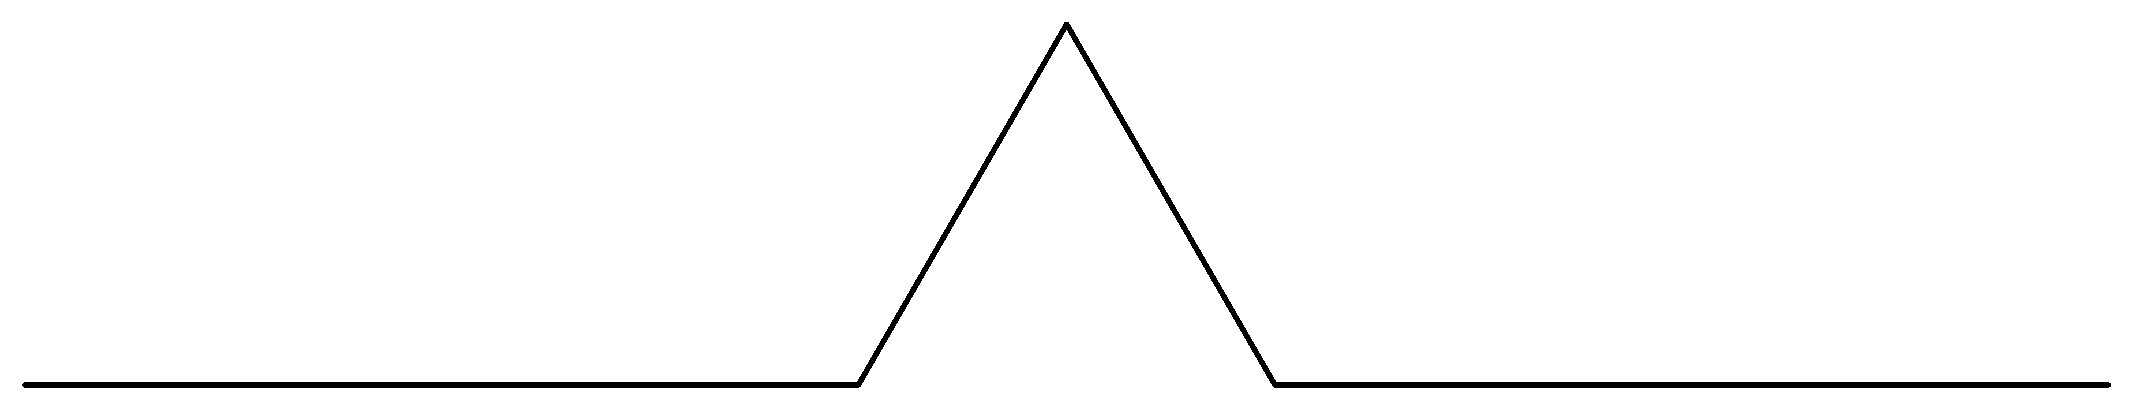
\includegraphics[width=\textwidth]{modified-koch-curve-iter1.pdf}
        \begin{center}
            $n=1$
        \end{center}
        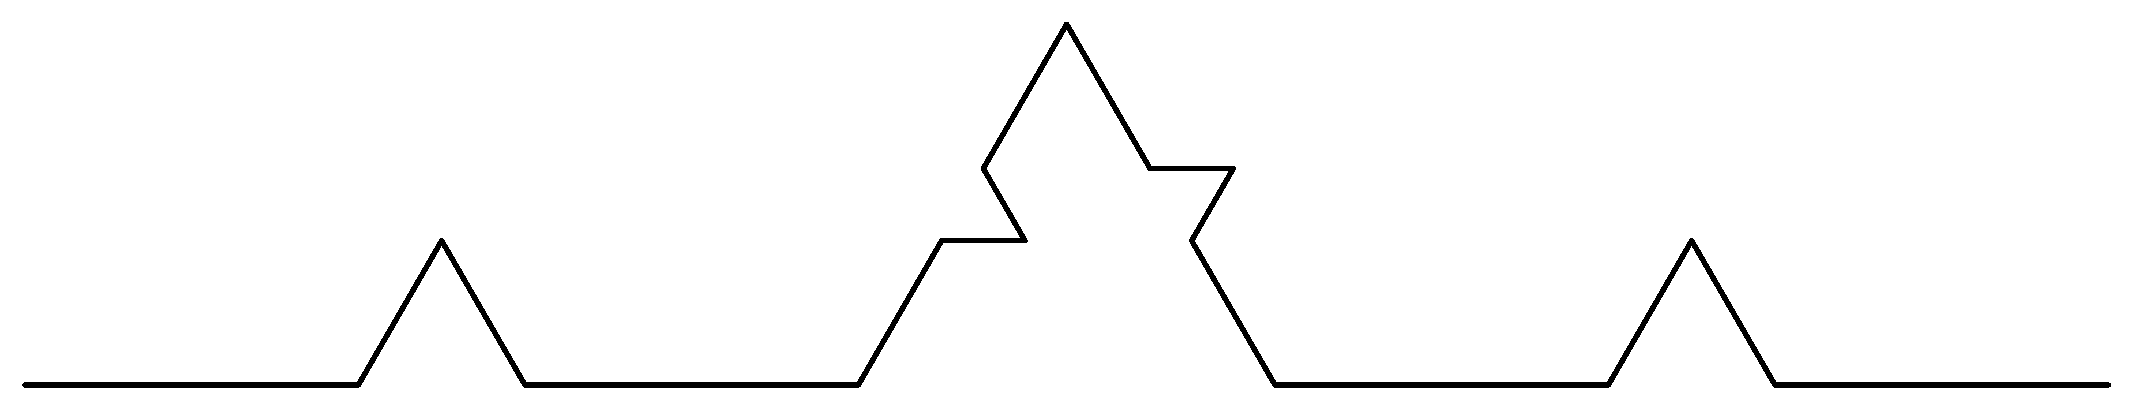
\includegraphics[width=\textwidth]{modified-koch-curve-iter2.pdf}
        \begin{center}
            $n=2$
        \end{center}
        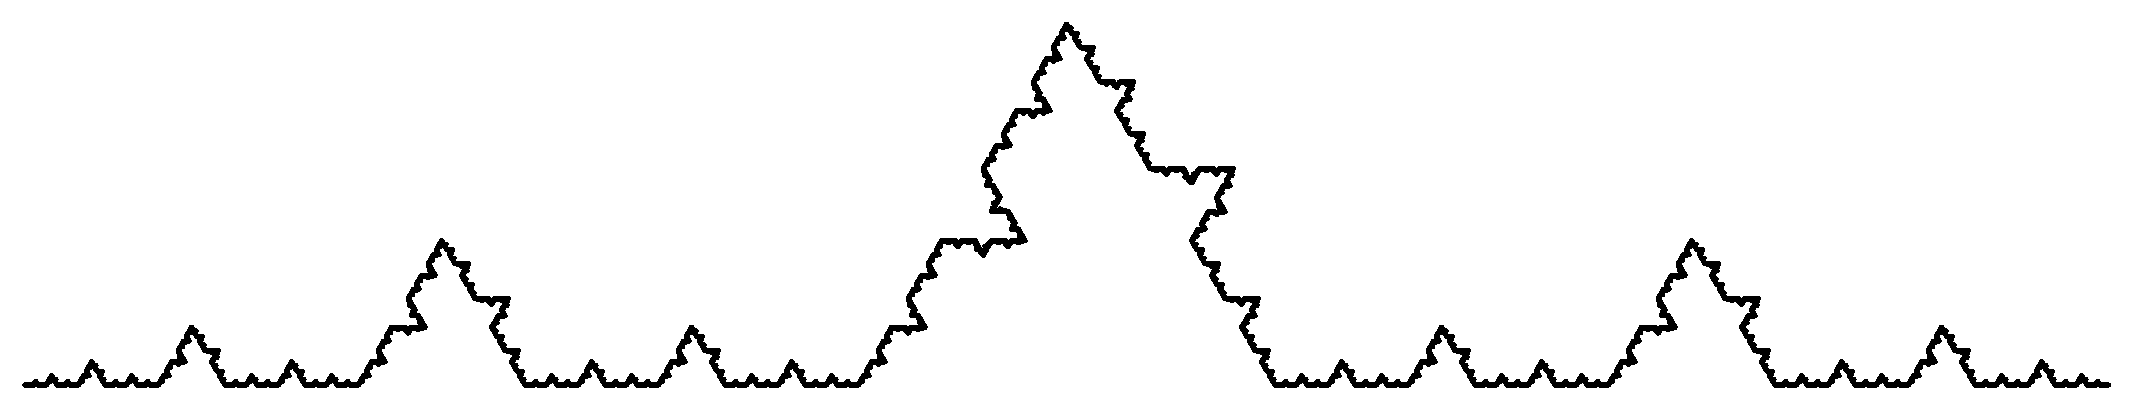
\includegraphics[width=\textwidth]{modified-koch-curve-iter6.pdf}
        \begin{center}
            $n=6$
        \end{center}
        \caption{Modifikovaná Kochova křivka pro $a=1/5$.}
        \label{fig:modifikovana-kochova-krivka}
    \end{figure}
    Označíme-li si opět faktory pro $\kappa_1,\kappa_2,\kappa_3$ a~$\kappa_4$ po řadě $r_1,r_2,r_3,r_4$, pak je zjevně
    \[r_1=r_2=\dfrac{1-a}{2},\;r_3=r_4=a.\]
    Tedy Hausdorffova dimenze, resp. box-counting dimenze $s$ je řešením rovnice
    \[2a^s+2\cdot\left(\dfrac{1-a}{2}\right)^s=1.\]
    Tu obecně algebraicky řešit nelze s~výjimkou $a=1/3$, což by byl případ standardní Kochovy křivky. Pro $a=1/5$ lze numericky dopočítat přibližné řešení $s\approx 1{,}1601$.
\end{example}
(Převzato a~upraveno z~\citep[str. 142]{Falconer1989}.)

Příklady výpočtů pro ostatní prezentované fraktální útvary si může čtenář vyzkoušet sám, neboť nejsou nikterak složité. V~některých případech může být obtížnější určit kontraktivní faktor daných zobrazení. Asi nejefektivější způsob (nechceme-li faktor počítat přímo z~definice) je přes tzv. \emph{SVD rozklad}\footnote{Zkratka pro \emph{Singular Value Decomposition}}\index{SVD roklad} a~\emph{singulární čísla}\footnote{Ta lze rovněž získat pomocí vlastních čísel matice $\mat{A}$.}\index{singulární číslo} matice $\mat{A}$. Tím se zde ale již zabývat nebudeme. Pro zvídavého čtenáře však doporučuji knihu \cite{Hladik2019}.